%%%%%%%%%%%%%%%%%%%%%%%%%%%%%%%%%%%%%%%%%%%%%%%%%%%%%%%%%%%%%%%%%%%%%%%%%%%%%%%%
%%%%%%%%%%%%%%%%%%%%%%%%%%%%%%%%%%%%%%%%%%%%%%%%%%%%%%%%%%%%%%%%%%%%%%%%%%%%%%%%
%
% Rechteinhaber:
%     Technische Universität München
%     https://www.tum.de
% 
% Gestaltung:
%     ediundsepp Gestaltungsgesellschaft, München
%     http://www.ediundsepp.de
% 
% Technische Umsetzung:
%     eWorks GmbH, Frankfurt am Main
%     http://www.eworks.de
%
%%%%%%%%%%%%%%%%%%%%%%%%%%%%%%%%%%%%%%%%%%%%%%%%%%%%%%%%%%%%%%%%%%%%%%%%%%%%%%%%


%%%%%%%%%%%%%%%%%%%%%%%%%%%%%%%%%%%%%%%%%%%%%%%%%%%%%%%%%%%%%%%%%%%%%%%%%%%%%%%%
% Zur Wahl des Seitenverhältnisses bitte einen der beiden folgenden Befehle
% auskommentieren und den ausführen lassen:
\documentclass[t]{beamer}
\usepackage[
    orientation=landscape,
    size=custom,
    width=25.4,
    height=19.05,
    scale=0.63 % erzeugt 16pt Schriftgröße
]{beamerposter}

\newcommand{\PraesentationSchriftgroesseSehrGross}{\fontsize{30}{45}}
\newcommand{\PraesentationSchriftgroesseGross}{\fontsize{22}{33}}
\newcommand{\PraesentationSchriftgroesseNormal}{\fontsize{16}{29}}
\newcommand{\PraesentationSchriftgroesseKlein}{\fontsize{12}{18}}
\newcommand{\PraesentationSchriftgroesseDreizeiler}{\fontsize{7}{10}}
\newcommand{\PraesentationSchriftgroesseAufzaehlungszeichen}{\fontsize{10}{8}}

\newcommand{\PraesentationAbstandAbsatz}{22.1pt}
\newcommand{\PraesentationPositionKorrekturOben}{0cm}
\newcommand{\PraesentationBeispieleSchriftgroessen}{30 | 22 | 16 | 12}
\usepackage[utf8]{inputenc}
\usepackage[T1]{fontenc} % Zeichensatzkodierung

\usepackage{calc} % Berechnungen

\usepackage[ngerman]{babel} % Deutsche Lokalisierung
\usepackage{graphicx} % Grafiken
\usepackage[export]{adjustbox}
\usepackage[absolute, overlay]{textpos} % Positionierung

% Silbentrennung:
\usepackage{hyphenat}
%\tolerance 2414
%\hbadness 2414
%\emergencystretch 1.5em
%\hfuzz 0.3pt
%\widowpenalty=10000     % Hurenkinder
%\clubpenalty=10000      % Schusterjungen
%\vfuzz \hfuzz

% Euro-Symbol:
\usepackage[gen]{eurosym}
\DeclareUnicodeCharacter{20AC}{\euro{}}

% Schriftart Helvetica:
\usepackage[scaled]{helvet}
\renewcommand{\familydefault}{\sfdefault}

\usepackage{mathptmx} % skalierbare Formelschriften

\usepackage{tabularx}

\usepackage{multicol} % mehrspaltiger Text

\usepackage{tikz}
\usetikzlibrary{arrows, shapes, shapes.multipart, trees, positioning,
    backgrounds, fit, matrix}

% Diagramme:
\usepackage{pgfplots}
\pgfplotsset{compat=default}

% Erweiterbare Fusszeile:
\newcommand{\PraesentationFusszeileZusatz}{}
 % Seitenverhältnis 4:3
% %\documentclass[aspectratio=169]{beamer}
\documentclass[t,aspectratio=169]{beamer}
\usepackage[
    orientation=landscape,
    size=custom,
    width=25.4,
    height=14.2875,
    scale=0.5
]{beamerposter}

\newcommand{\PraesentationSchriftgroesseSehrGross}{\fontsize{25}{38}}
\newcommand{\PraesentationSchriftgroesseGross}{\fontsize{18}{27}}
\newcommand{\PraesentationSchriftgroesseNormal}{\fontsize{14}{21}}
\newcommand{\PraesentationSchriftgroesseKlein}{\fontsize{11}{17}}
\newcommand{\PraesentationSchriftgroesseDreizeiler}{\fontsize{7}{10}}
\newcommand{\PraesentationSchriftgroesseAufzaehlungszeichen}{\fontsize{10}{8}}

\newcommand{\PraesentationAbstandAbsatz}{18pt}
\newcommand{\PraesentationPositionKorrekturOben}{-1cm}
\newcommand{\PraesentationBeispieleSchriftgroessen}{25 | 18 | 14 | 11}
\usepackage[utf8]{inputenc}
\usepackage[T1]{fontenc} % Zeichensatzkodierung

\usepackage{calc} % Berechnungen

\usepackage[ngerman]{babel} % Deutsche Lokalisierung
\usepackage{graphicx} % Grafiken
\usepackage[export]{adjustbox}
\usepackage[absolute, overlay]{textpos} % Positionierung

% Silbentrennung:
\usepackage{hyphenat}
%\tolerance 2414
%\hbadness 2414
%\emergencystretch 1.5em
%\hfuzz 0.3pt
%\widowpenalty=10000     % Hurenkinder
%\clubpenalty=10000      % Schusterjungen
%\vfuzz \hfuzz

% Euro-Symbol:
\usepackage[gen]{eurosym}
\DeclareUnicodeCharacter{20AC}{\euro{}}

% Schriftart Helvetica:
\usepackage[scaled]{helvet}
\renewcommand{\familydefault}{\sfdefault}

\usepackage{mathptmx} % skalierbare Formelschriften

\usepackage{tabularx}

\usepackage{multicol} % mehrspaltiger Text

\usepackage{tikz}
\usetikzlibrary{arrows, shapes, shapes.multipart, trees, positioning,
    backgrounds, fit, matrix}

% Diagramme:
\usepackage{pgfplots}
\pgfplotsset{compat=default}

% Erweiterbare Fusszeile:
\newcommand{\PraesentationFusszeileZusatz}{}
 % Seitenverhältnis 16:9
%%%%%%%%%%%%%%%%%%%%%%%%%%%%%%%%%%%%%%%%%%%%%%%%%%%%%%%%%%%%%%%%%%%%%%%%%%%%%%%%


%%%%%%%%%%%%%%%%%%%%%%%%%%%%%%%%%%%%%%%%%%%%%%%%%%%%%%%%%%%%%%%%%%%%%%%%%%%%%%%%
%%%%%%%%%%%%%%%%%%%%%%%%%%%%%%%%%%%%%%%%%%%%%%%%%%%%%%%%%%%%%%%%%%%%%%%%%%%%%%%%
% TUM-Vorlage: Personenspezifische Informationen
%%%%%%%%%%%%%%%%%%%%%%%%%%%%%%%%%%%%%%%%%%%%%%%%%%%%%%%%%%%%%%%%%%%%%%%%%%%%%%%%
%
% Rechteinhaber:
%     Technische Universität München
%     https://www.tum.de
% 
% Gestaltung:
%     ediundsepp Gestaltungsgesellschaft, München
%     http://www.ediundsepp.de
% 
% Technische Umsetzung:
%     eWorks GmbH, Frankfurt am Main
%     http://www.eworks.de
%
%%%%%%%%%%%%%%%%%%%%%%%%%%%%%%%%%%%%%%%%%%%%%%%%%%%%%%%%%%%%%%%%%%%%%%%%%%%%%%%%

% Für die Person anpassen:

\newcommand{\PersonTitel}{}
\newcommand{\PersonVorname}{Anton}
\newcommand{\PersonNachname}{Mai}
\newcommand{\PersonStadt}{München}
\newcommand{\PersonAdresse}{%
    @Adresse@\\%
    @Plz@~\PersonStadt%
}
\newcommand{\PersonTelefon}{@Telefon@}
\newcommand{\PersonFax}{@Fax@}
\newcommand{\PersonEmail}{@E-Mail@}
\newcommand{\PersonWebseite}{@Web@}

\newcommand{\FakultaetAnsprechpartner}{@Ansprechpartner@}
% Fakultät:
\newcommand{\FakultaetName}{Department of Informatics}
\newcommand{\LehrstuhlName}{Chair of Robotics, Artificial Intelligence and Real-time Systems}

\newcommand{\EinstellungBankName}{...}
\newcommand{\EinstellungBankIBAN}{...}
\newcommand{\EinstellungBankBIC}{...}
\newcommand{\EinstellungSteuernummer}{...}
\newcommand{\EinstellungUmsatzsteuerIdentifikationsnummer}{...}

\hyphenation{} % eigene Silbentrennung                    % !!! DATEI ANPASSEN !!!
%%%%%%%%%%%%%%%%%%%%%%%%%%%%%%%%%%%%%%%%%%%%%%%%%%%%%%%%%%%%%%%%%%%%%%%%%%%%%%%%


\renewcommand{\PersonTitel}{}
\newcommand{\Datum}{\today}

\renewcommand{\PraesentationFusszeileZusatz}{| RL for Robotic Arms}
\title{Reinforcement Learning for Path Planning of
	Robotic Arms}
\author{\PersonTitel{} \PersonVorname{} \PersonNachname}
\institute[]{\UniversitaetName \\ \FakultaetName \\ \LehrstuhlName}
\date[\Datum]{Munich, March 27th 2020}
\subject{Reinforcement Learning for Path Planning of
	Robotic Arms}


%%%%%%%%%%%%%%%%%%%%%%%%%%%%%%%%%%%%%%%%%%%%%%%%%%%%%%%%%%%%%%%%%%%%%%%%%%%%%%%%
%%%%%%%%%%%%%%%%%%%%%%%%%%%%%%%%%%%%%%%%%%%%%%%%%%%%%%%%%%%%%%%%%%%%%%%%%%%%%%%%
% EINSTELLUNGEN
%%%%%%%%%%%%%%%%%%%%%%%%%%%%%%%%%%%%%%%%%%%%%%%%%%%%%%%%%%%%%%%%%%%%%%%%%%%%%%%%

% Allgemein:
\newcommand{\AllgemeinGestalter}{ediundsepp Gestaltungsgesellschaft}
\newcommand{\AllgemeinErsteller}{eWorks GmbH}

% Universität:
\newcommand{\UniversitaetName}{Technische Universität München}
\newcommand{\UniversitaetAbkuerzung}{TUM}
\newcommand{\UniversitaetWebseite}{www.tum.de}
\newcommand{\UniversitaetLogoBreite}{19mm}
\newcommand{\UniversitaetLogoHoehe}{1cm}

\newcommand{\UniversitaetAdresse}{%
    Arcisstraße~21\\%
    80333~München%
}

\newcommand{\PraesentationSeitenrand}{8.9mm}
\newcommand\crule[3][black]{\textcolor{#1}{\rule{#2}{#3}}}

\newlength\smallerbaselineskip
\setlength{\smallerbaselineskip}{0.8\baselineskip}

    % Blautöne:
\definecolor{TUMBlau}{RGB}{0,101,189} % Pantone 300
\definecolor{TUMBlauDunkel}{RGB}{0,82,147} % Pantone 301
\definecolor{TUMBlauHell}{RGB}{152,198,234} % Pantone 283
\definecolor{TUMBlauMittel}{RGB}{100,160,200} % Pantone 542

    % Hervorhebung:
\definecolor{TUMElfenbein}{RGB}{218,215,203} % Pantone 7527 -Elfenbein
\definecolor{TUMGruen}{RGB}{162,173,0} % Pantone 383 - Grün
\definecolor{TUMOrange}{RGB}{227,114,34} % Pantone 158 - Orange
\definecolor{TUMGrau}{gray}{0.6} % Grau 60%


\setbeamercolor*{alerted text}{fg=TUMOrange}

\newcommand{\PraesentationSetzeTextfarbe}{%
    \color{PraesentationTextfarbe}%
    \setbeamercolor*{frametitle}{fg=PraesentationTextfarbe}%
    \setbeamercolor*{normal text}{fg=PraesentationTextfarbe}%
    \setbeamercolor{itemize/enumerate body}{fg=PraesentationTextfarbe}%
    \setbeamercolor*{itemize item}{fg=PraesentationTextfarbe}%
}

\newcommand{\PraesentationFarbschemaStandard}{%
    \setbeamercolor*{background canvas}{}%
    \definecolor{PraesentationTextfarbe}{rgb}{0,0,0}%
    \PraesentationSetzeTextfarbe%
}

\newcommand{\PraesentationFarbschemaWeissBlau}{%
    \setbeamercolor*{background canvas}{bg=TUMBlauDunkel}%
    \definecolor{PraesentationTextfarbe}{rgb}{1,1,1}%
    \PraesentationSetzeTextfarbe%
}

\newcommand{\PraesentationFarbschemaWeissSchwarz}{%
    \setbeamercolor*{background canvas}{bg=black}%
    \definecolor{PraesentationTextfarbe}{rgb}{1,1,1}%
    \PraesentationSetzeTextfarbe%
}

\newcommand{\PraesentationTitelseiteInhalt}{%
    \begin{textblock*}{\paperwidth}[0,0](0cm,-\PraesentationSeitenrand - 6.5mm + \PraesentationPositionKorrekturOben)%
        \color{PraesentationTextfarbe}%
        \frametitle{\inserttitle}
        \vspace*{59.4mm}%
        \usebeamerfont{author}\selectfont\insertauthor\\%
        \insertinstitute\\%
        \insertdate%
    \end{textblock*}%
}

\newcommand{\PraesentationSeitenkopfInhalt}[1]{%
    %\vspace*{31.7mm}%
    \begin{textblock*}{1.68cm}[1,0](\paperwidth - \PraesentationSeitenrand - \PraesentationSeitenrand, 0cm)%
        \includegraphics[width=1.68cm]{#1}%
    \end{textblock*}%
    \begin{textblock*}{3cm}[1,0](\paperwidth - \PraesentationSeitenrand, -\PraesentationSeitenrand)%
        \hbox{%
            \color{PraesentationTextfarbe}%
            \hbox{\insertframenavigationsymbol}%
            \hbox{\insertsubsectionnavigationsymbol}%
            \hbox{\insertsectionnavigationsymbol}%
        }%
    \end{textblock*}%
}

\newcommand{\PraesentationBildUhrenturm}{%
    \begin{textblock*}{10.82cm}[1,1](\paperwidth - \PraesentationSeitenrand - \PraesentationSeitenrand, \paperheight - 9mm)%
        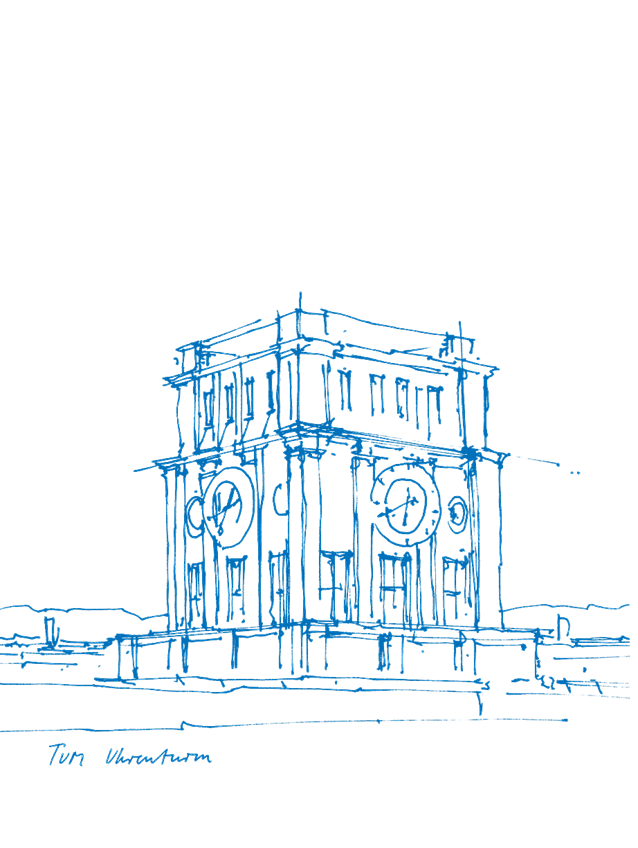
\includegraphics{./Ressourcen/Praesentation/Bilder/TUM_Uhrenturm.png}%
    \end{textblock*}%
}

\newcommand{\PraesentationStartseiteUhrenturm}{%
    \setbeamertemplate{title page}{%
        \PraesentationSeitenkopfInhalt{./Ressourcen/_Bilder/Universitaet_Logo_RGB.pdf}%
        \PraesentationBildUhrenturm%
        \PraesentationTitelseiteInhalt%
    }%
}

\newcommand{\PraesentationStartseiteFlaggen}{%
    \setbeamertemplate{title page}{%
        \begin{textblock*}{\paperwidth}[0,1](-\PraesentationSeitenrand,\paperheight-\PraesentationSeitenrand)%
            
\includegraphics[min width=\paperwidth,max width=\paperheight,min totalsize={\paperwidth}{\paperheight},keepaspectratio,center]{./Ressourcen/Praesentation/Bilder/Universitaet_Flaggen.jpg}%
        \end{textblock*}%
        \PraesentationSeitenkopfInhalt{./Ressourcen/_Bilder/Universitaet_Logo_weiss.pdf}%
        \PraesentationTitelseiteInhalt%
    }%
}

\newcommand{\PraesentationStartseiteLeer}{%
    \setbeamertemplate{title page}{%
        \PraesentationSeitenkopfInhalt{./Ressourcen/_Bilder/Universitaet_Logo_weiss.pdf}%
        \PraesentationTitelseiteInhalt%
    }%
}


\newcommand{\PraesentationMasterStandard}{%
    \PraesentationFarbschemaStandard%
    \PraesentationStartseiteUhrenturm%
    \setbeamertemplate{headline}{%
        \PraesentationSeitenkopfInhalt{./Ressourcen/_Bilder/Universitaet_Logo_RGB.pdf}%
    }%
}

\newcommand{\PraesentationMasterWeissBlau}{%
    \PraesentationFarbschemaWeissBlau%
    \PraesentationStartseiteLeer%
    \setbeamertemplate{headline}{%
        \PraesentationSeitenkopfInhalt{./Ressourcen/_Bilder/Universitaet_Logo_weiss.pdf}%
    }%
}


\newcommand{\PraesentationMasterKopfzeileDreizeiler}{%
    \PraesentationFarbschemaStandard%
    \setbeamertemplate{title page}{%
        \begin{textblock*}{\paperwidth}[0,0](0cm, -7.8mm)%
            \color{TUMBlau}\PraesentationSchriftgroesseDreizeiler\selectfont%
            \LehrstuhlName\\%
            \FakultaetName\\%
            \UniversitaetName\vskip0pt%
            \normalcolor\normalsize\selectfont%
        \end{textblock*}%
        \PraesentationSeitenkopfInhalt{./Ressourcen/_Bilder/Universitaet_Logo_RGB.pdf}%
        \PraesentationBildUhrenturm%
        \PraesentationTitelseiteInhalt%
    }%
    \setbeamertemplate{headline}{%
        \begin{textblock*}{\paperwidth}[0,0](0cm, 0cm)%
            \begin{minipage}[t][2cm][t]{\paperwidth}%
                \color{TUMBlau}\PraesentationSchriftgroesseDreizeiler\selectfont%
                \LehrstuhlName\\[1.38mm]%
                \FakultaetName\\[1.44mm]%
                \UniversitaetName\vskip0pt%
                \normalcolor\normalsize\selectfont%
            \end{minipage}%
        \end{textblock*}%
        \PraesentationSeitenkopfInhalt{./Ressourcen/_Bilder/Universitaet_Logo_RGB.pdf}%
    }%
}

\newcommand{\PraesentationMasterWeissSchwarz}{%
    \PraesentationFarbschemaWeissSchwarz%
    \setbeamertemplate{title page}{%
        \PraesentationTitelseiteInhalt%
        \PraesentationSeitenkopfInhalt{./Ressourcen/_Bilder/Universitaet_Logo_weiss.pdf}%
    }
    \setbeamertemplate{headline}{%
        \PraesentationSeitenkopfInhalt{./Ressourcen/_Bilder/Universitaet_Logo_weiss.pdf}%
    }
}

\newcommand{\PraesentationTitelseite}{\frame[plain]{\titlepage}}
\newcommand{\PraesentationUeberschriftZweizeilig}[2]{\frametitle{#1\\[8mm]#2}}

\setbeamersize{
    text margin left=\PraesentationSeitenrand,
    text margin right=\PraesentationSeitenrand
}

\setbeamertemplate{frametitle}{%
    {\rule{0pt}{42mm + \PraesentationPositionKorrekturOben}\PraesentationSchriftgroesseSehrGross\selectfont\insertframetitle\newline\vspace*{-6.7mm}}%
}

% Aufzählungen:
\newcommand{\PraesentationAufzaehlungEbeneEinsSymbol}{\raise2pt\hbox{\donotcoloroutermaths\usebeamercolor{itemize subitem}\PraesentationSchriftgroesseAufzaehlungszeichen$\bullet$}}
\newcommand{\PraesentationAufzaehlungEbeneZweiSymbol}{\raise1.25pt\hbox{\donotcoloroutermaths\usebeamercolor{itemize subitem}$-$}}
\setbeamertemplate{itemize items}[circle]
\setbeamertemplate{itemize subitem}[triangle]
\setbeamercolor{itemize subitem}{fg=black}
\setbeamerfont{itemize/enumerate subbody}{size=\normalsize}
\setbeamertemplate{itemize item}{\PraesentationAufzaehlungEbeneEinsSymbol}
\setbeamertemplate{itemize subitem}{\PraesentationAufzaehlungEbeneZweiSymbol{}}
%\addtolength{\leftmarginii}{16mm-2pt}%

\newenvironment{PraesentationAufzaehlung}
{%
    \vspace{-\baselineskip}%
    \begin{itemize}%
        \setlength{\itemsep}{0pt}%
        \setlength{\parskip}{0pt}%
        \setlength{\parsep}{0pt}%
        \addtolength{\itemindent}{-1ex}%
}{%
    \end{itemize}%
}

%%%%%%%%%%%%%%%%%%%%%%%%%%%%%%%%%%%%%%%%%%%%%%%%%%%%%%%%%%%%%%%%%%%%%%%%%%%%%%%%
% DOKUMENT
%%%%%%%%%%%%%%%%%%%%%%%%%%%%%%%%%%%%%%%%%%%%%%%%%%%%%%%%%%%%%%%%%%%%%%%%%%%%%%%%


% PDF-Einstellungen:
\hypersetup{
    pdfstartview={Fit},
    pdfproducer={\AllgemeinErsteller},
    pdfcreator={\AllgemeinGestalter}
}

\textblockorigin{\PraesentationSeitenrand}{\PraesentationSeitenrand} % Ursprung für Positionierung

\setbeamerfont{footnote}{size=\PraesentationSchriftgroesseKlein}

\setbeamertemplate{footline}{
    \hbox{%
        \usebeamerfont{footnote}%
        \begin{beamercolorbox}[wd=.9\paperwidth]{}%
            \hspace*{\PraesentationSeitenrand}%
            \PersonTitel{} \PersonVorname~\PersonNachname~(\UniversitaetAbkuerzung) \PraesentationFusszeileZusatz{}%
        \end{beamercolorbox}%
        \begin{beamercolorbox}[wd=.1\paperwidth]{}%
            \insertframenumber{}%
            \raggedleft
            \hspace*{\PraesentationSeitenrand}%
        \end{beamercolorbox}%
        \vspace*{3.25mm}%
    }%
}

\setbeamertemplate{navigation symbols}{}

\begin{document}
\setlength{\baselineskip}{\PraesentationAbstandAbsatz}
\setlength{\parskip}{\baselineskip}
 % !!! NICHT ENTFERNEN !!!
%%%%%%%%%%%%%%%%%%%%%%%%%%%%%%%%%%%%%%%%%%%%%%%%%%%%%%%%%%%%%%%%%%%%%%%%%%%%%%%%


%%%%%%%%%%%%%%%%%%%%%%%%%%%%%%%%%%%%%%%%%%%%%%%%%%%%%%%%%%%%%%%%%%%%%%%%%%%%%%%%
% !!!ÄNDERUNG HIER:!!!
\PraesentationMasterStandard

\PraesentationTitelseite % Fügt die Startseite ein


%%%%%%%%%%%%%%%%%%%%%%%%%%%%%%%%%%%%%%%%%%%%%%%%%%%%%
%% Beispielfolien                                  %%
%%%%%%%%%%%%%%%%%%%%%%%%%%%%%%%%%%%%%%%%%%%%%%%%%%%%%%%%%%%%%%%%%%%%%%%%%%%%%%%%%
% TUM-Vorlage: Präsentation - Beispiele
%%%%%%%%%%%%%%%%%%%%%%%%%%%%%%%%%%%%%%%%%%%%%%%%%%%%%%%%%%%%%%%%%%%%%%%%%%%%%%%%


%%%%%%%%%%%%%%%%%%%%%%%%%%%%%%%%%%%%%%%%%%%%%%%%%%%%%
%% Folie: Gültigkeit der Masterfolien              %%
%%%%%%%%%%%%%%%%%%%%%%%%%%%%%%%%%%%%%%%%%%%%%%%%%%%%%

\begin{frame}
    \frametitle{Gültigkeit der Masterfolien}

Dieser Folienmaster gilt bei offiziellen Präsentationen im Rahmen der TUM. Es
ist darauf zu achten, dass wir uns in einem durchgängigen Layout präsentieren.

Abweichungen vom vorgegebenen Layout bitte auf ein Minimum reduzieren.

\end{frame}
\clearpage


%%%%%%%%%%%%%%%%%%%%%%%%%%%%%%%%%%%%%%%%%%%%%%%%%%%%%
%% Folie: Grundlage der Masterfolien               %%
%%%%%%%%%%%%%%%%%%%%%%%%%%%%%%%%%%%%%%%%%%%%%%%%%%%%%

\begin{frame}
    \frametitle{Grundlage der Masterfolien}

Als Grundlage dient der Corporate Design Style Guide der TUM.\newline
Die Präsentationsvorlage ist auf gute Lesbarkeit und klare Darstellung von
Informationen optimiert.

\end{frame}
\clearpage


%%%%%%%%%%%%%%%%%%%%%%%%%%%%%%%%%%%%%%%%%%%%%%%%%%%%%
%% Folie: 2-zeilige Überschrift                    %%
%%%%%%%%%%%%%%%%%%%%%%%%%%%%%%%%%%%%%%%%%%%%%%%%%%%%%

\begin{frame}
    \PraesentationUeberschriftZweizeilig{Hier steht eine}{2-zeilige Überschrift}

Als Grundlage dient der Corporate Design Style Guide der TUM.\newline
Die Präsentationsvorlage ist auf gute Lesbarkeit und klare Darstellung von
Informationen optimiert.

\end{frame}
\clearpage


%%%%%%%%%%%%%%%%%%%%
%% Folie: Schrift %%
%%%%%%%%%%%%%%%%%%%%
\begin{frame}
    \frametitle{Schrift}

Das Grundprinzip ist, Informationen bestmöglich zu transportieren. Dazu muss
vor allem die Schrift einheitlich und für alle im Raum lesbar sein.

Schriftart: Helvetica

Schriftgößen: \PraesentationBeispieleSchriftgroessen

Zeilenabstand: 1,15 mm

Die Einstellungen sind für diese Vorlage als Standard eingestellt. Bei
Diagrammen und Tabellen muss die Schriftgröße ggf. angepasst werden. Für
Ausszeichnungen im Fließtext kann auch \textbf{fett} markiert werden. Bei
großer Distanz bzw. kleinem Präsenationsmedium kann der Schriftgrad notfalls
proportional erhöht werden.

\end{frame}
\clearpage


%%%%%%%%%%%%%%%%%%%
%% Folie: Farben %%
%%%%%%%%%%%%%%%%%%%
\begin{frame}
    \frametitle{Farben}
    
Als erstes soll mit schwarz und weiß gearbeitet werden.\newline
Für Aufwändigere Darstellungen sind Farben mit Bedacht und in möglichst
geringem Umfang einzusetzen.

In diesem Folienmaster ist die Farbpalette festgelegt.

{
    \renewcommand{\arraystretch}{1.2} % skaliert die Tabellen mit Farbfeldern

    Zuerst mit den Primärfarben arbeiten.

    \setlength{\fboxsep}{-1pt} \setlength{\fboxrule}{1pt} % fbox/framebox konfigurieren

    \vspace*{-5mm}
    \begin{tabularx}{\textwidth}{@{} l @{\hspace{4mm}} l @{\hspace{4mm}} l}
        \crule[TUMBlau]{24mm}{6mm}
        & \crule[black]{24mm}{6mm}
        & \fbox{\crule[white]{24mm}{6mm}}
    \end{tabularx}

    \vspace*{-5mm}
    Für z.B. komplexe Diagramme stehen noch Sekundärfarben zur Verfügung.

    \vspace*{-5mm}
    \begin{tabularx}{\textwidth}{@{} l @{\hspace{4mm}} l @{\hspace{4mm}} l @{\hspace{4mm}} l}
        \crule[TUMBlauDunkel]{24mm}{6mm}
        & \crule[TUMBlauMittel]{24mm}{6mm}
        & \crule[TUMBlauHell]{24mm}{6mm}
        & \crule[TUMGrau]{24mm}{6mm}
    \end{tabularx}

    \vspace*{-5mm}
    Bei weiterer Komplexität oder zusätzlichen Markierungen:

    \vspace*{-5mm}
    \begin{tabularx}{\textwidth}{@{} l @{\hspace{4mm}} l @{\hspace{4mm}} l }
        \crule[TUMOrange]{24mm}{6mm}
        & \crule[TUMGruen]{24mm}{6mm}
        & \crule[TUMElfenbein]{24mm}{6mm}
    \end{tabularx}
}

\end{frame}
\clearpage


%%%%%%%%%%%%%%%%%%
%% Folie: Texte %%
%%%%%%%%%%%%%%%%%%
\begin{frame}
    \frametitle{Texte}
 
Kurze und knappe Texte, Fließtexte linksbündig, kein Blocksatz \\[\baselineskip]

Beispiel:\newline
Tem soluptam, nisi as verum ereprehendam at acculpa quidisq uissit volupta
tusdant utem as etur, odi odis es doluptiae dem nimaion con nossinctenis pora
quam voloria consenimus blabore everfer epeliquo maio etur.

\end{frame}
\clearpage


%%%%%%%%%%%%%%%%%%%%%%%
%% Folie: Aufzählung %%
%%%%%%%%%%%%%%%%%%%%%%%
\begin{frame}
    \frametitle{Aufzählung}
    
Bei kleinen Aufzählungen auf Aufzählungszeichen verzichten und ggf. zusätzliche Leerzeile.\newline
Nur die wesentlichen Punkte nennen und Themen auf verschiedene Seiten splitten.\\
Punkt 1\\
Punkt 2

Wenn Unterpunkte in einer Aufzählung nötig sind ist ein Einrücken mit \PraesentationAufzaehlungEbeneZweiSymbol{} möglich

\begin{PraesentationAufzaehlung}
    \item Unterpunkt 1
        \begin{itemize}
            \item Unterpunkt 1
            \item Unterpunkt 2
        \end{itemize}
\end{PraesentationAufzaehlung}

Bei größeren Listen die Standardeinstellung \PraesentationAufzaehlungEbeneEinsSymbol{} verwenden

\begin{PraesentationAufzaehlung}
    \item Unterpunkt 1
    \item Unterpunkt 2
    \item Unterpunkt 3
\end{PraesentationAufzaehlung}

\end{frame}
\clearpage


%%%%%%%%%%%%%%%%%%%%%%%%%%%%%%%
%% Folie: Bilder - Allgemein %%
%%%%%%%%%%%%%%%%%%%%%%%%%%%%%%%
\begin{frame}
    \frametitle{Bilder -- Allgemein}
    
schlichte Darstellung von Informationen \\[\baselineskip]

reduzierte Farben \\[\baselineskip]

Rahmen und Überlagerungen nach Möglichkeit vermeiden \\[\baselineskip]

    
\end{frame}
\clearpage


%%%%%%%%%%%%%%%%%%%%%%%%%%
%% Folie: Bilder - Zwei %%
%%%%%%%%%%%%%%%%%%%%%%%%%%
\begin{frame}
    \frametitle{Bilder}
    
Bildbeschreibung\newline
oberer Bildrand: Begrenzung durch Text\\[\baselineskip]

\mbox{
\includegraphics[height=.5\paperheight, trim=0cm 14cm 0cm 0cm, clip=true]{./Ressourcen/_Bilder/SternenhimmelHochkant.jpg}}%
\hspace{6.5mm}%
\mbox{
\includegraphics[height=.5\paperheight, trim=0cm 14cm 0cm 0cm, clip=true]{./Ressourcen/_Bilder/SternenhimmelHochkant.jpg}}

\end{frame}
\clearpage


%%%%%%%%%%%%%%%%%%%%%%%%%%%%%%%%%%%%%%%%
%% Folie: Bilder - Zweispaltige Seite %%
%%%%%%%%%%%%%%%%%%%%%%%%%%%%%%%%%%%%%%%%
\begin{frame}
    \frametitle{Bilder}

\begin{multicols}{2}
    \textbf{Überschrift 2}\newline
    Hier steht ein einleitender oder beschreibender Fließtext und nach Wunsch
    eine Aufzählung.

    Punkt 1

    Punkt 2

    Punkt 3

    Punkt 4
    \vfill\columnbreak
    
\includegraphics[width=\columnwidth, height=.7\textheight]{./Ressourcen/_Bilder/SternenhimmelHochkant.jpg}%
\end{multicols}
    
\end{frame}
\clearpage


%%%%%%%%%%%%%%%%%%%%%%%%%%%%%%%
%% Folie: Bilder - Textbreit %%
%%%%%%%%%%%%%%%%%%%%%%%%%%%%%%%
\begin{frame}
    \frametitle{Bilder}

Bildbeschreibung\newline
oberer Bildrand: Begrenzung durch Text\\[\baselineskip]


\includegraphics[width=\textwidth, height=.55\textheight]{./Ressourcen/_Bilder/SternenhimmelQuer.jpg}%

\end{frame}
\clearpage


%%%%%%%%%%%%%%%%%%%%%%%%%%%%%%%%%%%%%%%%%%%%%%%%%%
%% Folie: Bilder - seitenbreit mit Beschreibung %%
%%%%%%%%%%%%%%%%%%%%%%%%%%%%%%%%%%%%%%%%%%%%%%%%%%
\begin{frame}
    \frametitle{Bilder}

    Bildbeschreibung\newline
    oberer Bildrand: Begrenzung durch Text

\vspace*{-3mm}
\begin{minipage}[t][0cm]{\paperwidth}%
\hspace*{-\PraesentationSeitenrand}%

\includegraphics[width=\paperwidth]{./Ressourcen/_Bilder/SternenhimmelQuer.jpg}
\end{minipage}
    
\end{frame}
\clearpage


%%%%%%%%%%%%%%%%%%%%%%%%%%%%%%%%%%%%%%%%%%%%%%%%%%%%%
%% Folie: Nicht Format füllende Bilder %%
%%%%%%%%%%%%%%%%%%%%%%%%%%%%%%%%%%%%%%%%%%%%%%%%%%%%%
\begin{frame}
    \frametitle{Nicht Format füllende Bilder}
    
    Weißer bzw. transparenter Hintergrund\newline
    mit genug Freiraum anordnen


\begin{textblock*}{0.4\paperwidth}[0,1](0cm, \textheight - \PraesentationSeitenrand)%
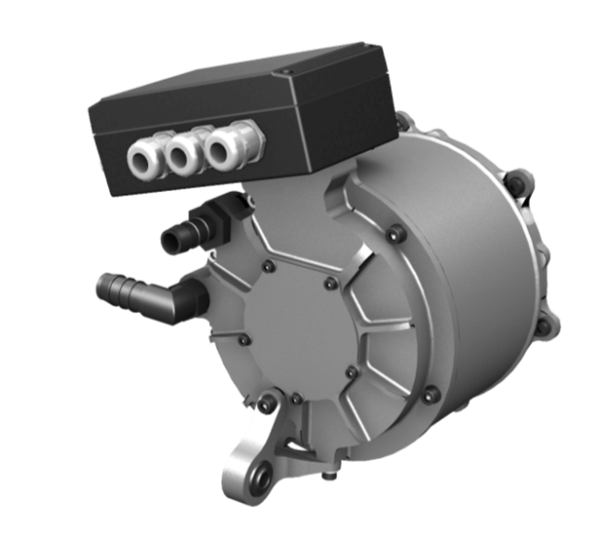
\includegraphics[width=0.4\paperwidth]{./Ressourcen/Praesentation/Bilder/Motor.png}
\end{textblock*}

\begin{textblock*}{0.6\paperwidth}[1,1](\textwidth + \PraesentationSeitenrand, \textheight - \PraesentationSeitenrand)%
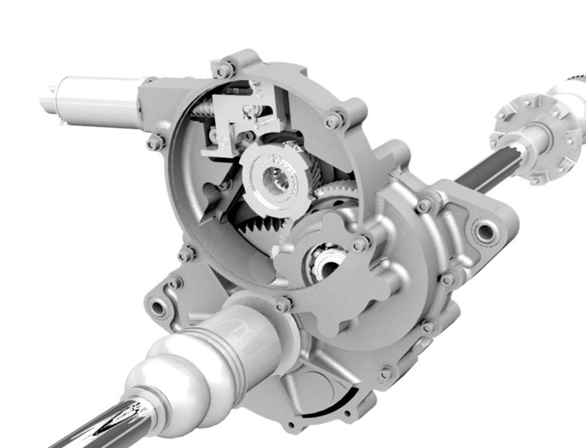
\includegraphics[width=0.6\paperwidth]{./Ressourcen/Praesentation/Bilder/Getriebe.png}
\end{textblock*}

\end{frame}
\clearpage


%%%%%%%%%%%%%%%%%%%%%%%%%%%%%%%%%%%
%% Folie: Bilder - formatfüllend %%
%%%%%%%%%%%%%%%%%%%%%%%%%%%%%%%%%%%
\begin{frame}
    \frametitle{Bilder Format füllend -- maximale Bildgröße}

\begin{minipage}[t][0cm]{\paperwidth}%
\hspace*{-\PraesentationSeitenrand}%

\includegraphics[width=\textwidth]{./Ressourcen/_Bilder/SternenhimmelQuer.jpg}
\end{minipage}
    
\end{frame}
\clearpage


%%%%%%%%%%%%%%%%%%%%%%%%%%%%%%%%%%%%%%%%%%%%%%%%%%%%%
%% Folie: Nicht Format füllende Bilder %%
%%%%%%%%%%%%%%%%%%%%%%%%%%%%%%%%%%%%%%%%%%%%%%%%%%%%%
\begin{frame}
    \frametitle{Nicht Format füllende Bilder}
    
Alternativ mit formatfüllendem Hintergrund: Weiß 5\% dunkler\newline
Beschriftungen können zusätzlich neben den Bildern angebracht werden

\begin{textblock*}{\paperwidth}[0,0](0cm, .4\textheight)%
Bilderklärung
\end{textblock*}

\begin{textblock*}{\paperwidth}[1,0](\textwidth, .4\textheight)%
\raggedleft%
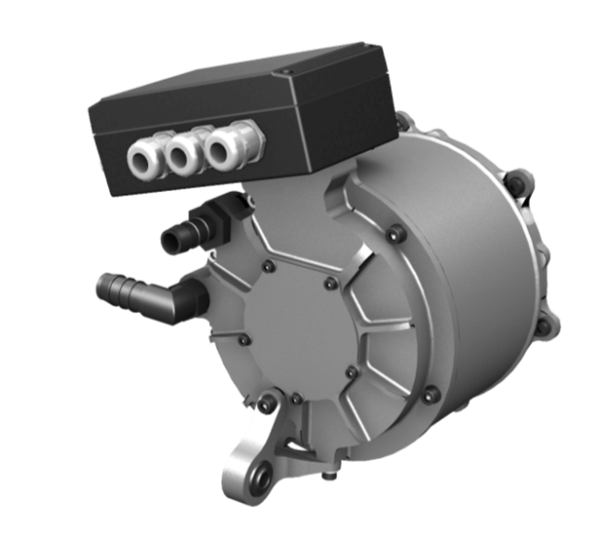
\includegraphics[height=0.5\textheight]{./Ressourcen/Praesentation/Bilder/Motor.png}
\end{textblock*}

\end{frame}
\clearpage


%%%%%%%%%%%%%%%%%%%%%%%%%%%%%%%%%%%%%%%%%%%%%%%%%%%%%
%% Folie: Tabelle - Ohne Rand 					   %%
%%%%%%%%%%%%%%%%%%%%%%%%%%%%%%%%%%%%%%%%%%%%%%%%%%%%%
\begin{frame}
    \frametitle{Tabelle -- Beispiel 1}
    
Tabelle ohne Farbe und kein Rand \\
innerer Seitenrand links 0 cm, um Faktor 1,75 skalierte Tabelle (für genug Zeilenabstand)

\raggedright
{
    \vspace*{0.3pt}
    \renewcommand{\arraystretch}{1.75} % skaliert die Tabelle auf die gewünschte Größe
    \begin{tabularx}{\textwidth}{@{} l @{\hspace{38.7mm}} l}
        Ø - Strecke & 39 km/Tag (14.360 km/Jahr) \\
        Ø - Geschwindigkeit & 25 km/h \\
        Ø - Verfügbare Ladezeit & 22 h/Tag \\
        Kosten   & Kleinwagen mit Verbrennungsmotor \\
        Einsatzgebiet   &  Stadt und Umland
    \end{tabularx}
}
\end{frame}


%%%%%%%%%%%%%%%%%%%%%%%%%%%%%%%%%%%%%%%%%%%%%%%%%%%%%
%% Folie: Tabelle - Mit Rand                       %%
%%%%%%%%%%%%%%%%%%%%%%%%%%%%%%%%%%%%%%%%%%%%%%%%%%%%%
\begin{frame}
    \frametitle{Tabelle -- Beispiel 2}
    
Tabelle ohne Farbe und mit Rand\\
automatische Zelleninnenabstände, um Faktor 1,75 skalierte Tabelle (für genug Zeilenabstand)

\raggedright
{
    \vspace*{0.3pt}
    \renewcommand{\arraystretch}{1.75} % skaliert die Tabelle auf die gewünschte Größe
    \begin{tabularx}{\textwidth}{| l @{\hspace{38.7mm}} | X |}
        \hline
        Ø - Strecke & 39 km/Tag (14.360 km/Jahr) \\ \hline
        Ø - Geschwindigkeit & 25 km/h \\ \hline
        Ø - Verfügbare Ladezeit & 22 h/Tag \\ \hline
        Kosten   & Kleinwagen mit Verbrennungsmotor \\ \hline
        Einsatzgebiet   &  Stadt und Umland \\ \hline
    \end{tabularx}
}
\end{frame}

\clearpage


%%%%%%%%%%%%%%%%%%%%%%%%%%%%%%%%%%%%%%%%%%%%%%%%%%%%%
%% Folie: Diagramme - Beispiel 1                   %%
%%%%%%%%%%%%%%%%%%%%%%%%%%%%%%%%%%%%%%%%%%%%%%%%%%%%%
\begin{frame}
    \frametitle{Diagramme -- Beispiel 1}

Nach Möglichkeit linksbündig bleiben \\
Unnötige Striche und Balken vermeiden

\begin{center}%
    \vspace*{-1cm}
    \begin{tikzpicture}
        \begin{axis}[
                % kein Abstand zwischen Balken:
                xbar=0,
                draw opacity=0,
                bar width=14,
                axis x line=none,
                axis line style={transparent},
                every tick/.style={transparent},
                xmin=0,
                width=\textwidth,
                height=.6\textheight,
                enlarge y limits=0.15,
                symbolic y coords={Kategorie 4,Kategorie 3,Kategorie 2,Kategorie 1},
                ytick=data,
                legend image code/.code={\draw[draw=none] (0cm,-0.12cm) rectangle (0.29cm,0.17cm);}, % Legenden-Symbol  
                legend columns=3,
                reverse legend,
                legend style={
                    fill=none,
                    draw=none,
                    /tikz/every odd column/.append style={column sep=0.07cm}, % Abstand zwischen Legenden-Symbol und Text
                    /tikz/every even column/.append style={column sep=0.8cm} % Abstand zwischen den Legendeneinträgen
                 },
                 legend to name=PraesentationDiagrammHorizontalLegende
            ]
            
            \addlegendentry{Datenreihe 3}
            \addlegendentry{Datenreihe 2}
            \addlegendentry{Datenreihe 1}
            
            \addplot[color=TUMBlauMittel, fill=TUMBlauMittel] coordinates {
                (1.2,Kategorie 1)
                (1.6,Kategorie 2)
                (2.2,Kategorie 3)
                (3.4,Kategorie 4)
            };
            
            \addplot[color=TUMBlauHell, fill=TUMBlauHell] coordinates {
                (1.5,Kategorie 1)
                (3.0,Kategorie 2)
                (1.0,Kategorie 3)
                (2.0,Kategorie 4)
            };
                
            \addplot[color=TUMBlauDunkel, fill=TUMBlauDunkel] coordinates {
                (3.0,Kategorie 1)
                (2.0,Kategorie 2)
                (2.5,Kategorie 3)
                (3.0,Kategorie 4)
            };
        \end{axis}
    \end{tikzpicture}

    \vspace*{-5mm}
    \ref*{PraesentationDiagrammHorizontalLegende}%
\end{center}
\end{frame}
\clearpage


%%%%%%%%%%%%%%%%%%%%%%%%%%%%%%%%%%%%%%%%%%%%%%%%%%%%%
%% Folie: Diagramme                                %%
%%%%%%%%%%%%%%%%%%%%%%%%%%%%%%%%%%%%%%%%%%%%%%%%%%%%%
\begin{frame}
    \frametitle{Diagramme}

\begin{center}
    \begin{tikzpicture}
        \begin{axis}[
                ybar=9.5,
                bar width=27.1,
                axis line style={transparent},
                every tick/.style={transparent},
                enlarge x limits=0.145, % X-Achse skalieren
                clip limits=true,
                ymin=0,
                ymax=6,
                width=\textwidth,
                height=.65\textheight,
                symbolic x coords={Kategorie 1,Kategorie 2,Kategorie 3,Kategorie 4},
                xticklabels={Kategorie 1,Kategorie 2,Kategorie 3,Kategorie 4},
                xtick=data,
                ytick={0,1,2,3,4,5,6},
                every tick label/.append style={font=\fontsize{13}{14}\selectfont},
                ymajorgrids,
                legend image code/.code={\draw[draw=none] (0cm,-0.12cm) rectangle (0.29cm,0.17cm);}, % Legenden-Symbol  
                legend columns=3,
                reverse legend,
                legend style={
                    font={\usebeamerfont{footnote}},
                    fill=none,
                    draw=none,
                    /tikz/every odd column/.append style={column sep=0.07cm}, % Abstand zwischen Legenden-Symbol
                    /tikz/every even column/.append style={column sep=0.8cm} % Abstand zwischen den Legendeneinträgen
                 },
                legend to name=PraesentationDiagrammVertikalLegende
            ]
            
            \addlegendentry{Datenreihe 3}        
            \addlegendentry{Datenreihe 2}    
            \addlegendentry{Datenreihe 1}    
            
            \addplot[color=TUMBlauDunkel, fill=TUMBlauDunkel] coordinates {
                (Kategorie 1,4.2)
                (Kategorie 2,2.5)
                (Kategorie 3,3.5)
                (Kategorie 4,4.5)
            };
            
            \addplot[color=TUMBlauHell, fill=TUMBlauHell] coordinates {
                (Kategorie 1,2.3)
                (Kategorie 2,4.5)
                (Kategorie 3,1.8)
                (Kategorie 4,2.8)
            };
            
            \addplot[color=TUMBlauMittel, fill=TUMBlauMittel] coordinates {
                (Kategorie 1,2.0)
                (Kategorie 2,2.0)
                (Kategorie 3,3.0)
                (Kategorie 4,5.0)
            };        
        \end{axis}
    \end{tikzpicture}

    \vspace*{-5mm}
    \ref*{PraesentationDiagrammVertikalLegende}%
\end{center}
\end{frame}
\clearpage


%%%%%%%%%%%%%%%%%%%%%%%%%%%%%%%%%%%%%%%%%%%%%%%%%%%%%


%%%%%%%%%%%%%%%%%%%%%%%%%%%%%%%%%%%%%%%%%%%%%%%%%%%%%%%%%%%%%%%%%%%%%%%%%%%%%%%%
% Kopfbereich links
\PraesentationMasterKopfzeileDreizeiler

\PraesentationTitelseite



%%%%%%%%%%%%%%%%%%%%%%%%%%%%%%%%%%%%%%%%%%%%%%%%%%%%%%%%%%%%%%%%%%%%%%%%%%%%%%%%

%TODO change some texts, replace the graphs


% Seite 1


%%%%%%%%%%%%%%%%%%%%%%%%%%%%%%%%%%%%%%%%%%%%%%%%%%%%%%%%%%%%%%%%%%%%%%%%%%%%%%%%

\begin{frame}
	\frametitle{Motivation}	
	\vspace{1cm}
	
	\begin{textblock*}{0.4\paperwidth}[0,1](0cm, 16cm - \PraesentationSeitenrand)%
		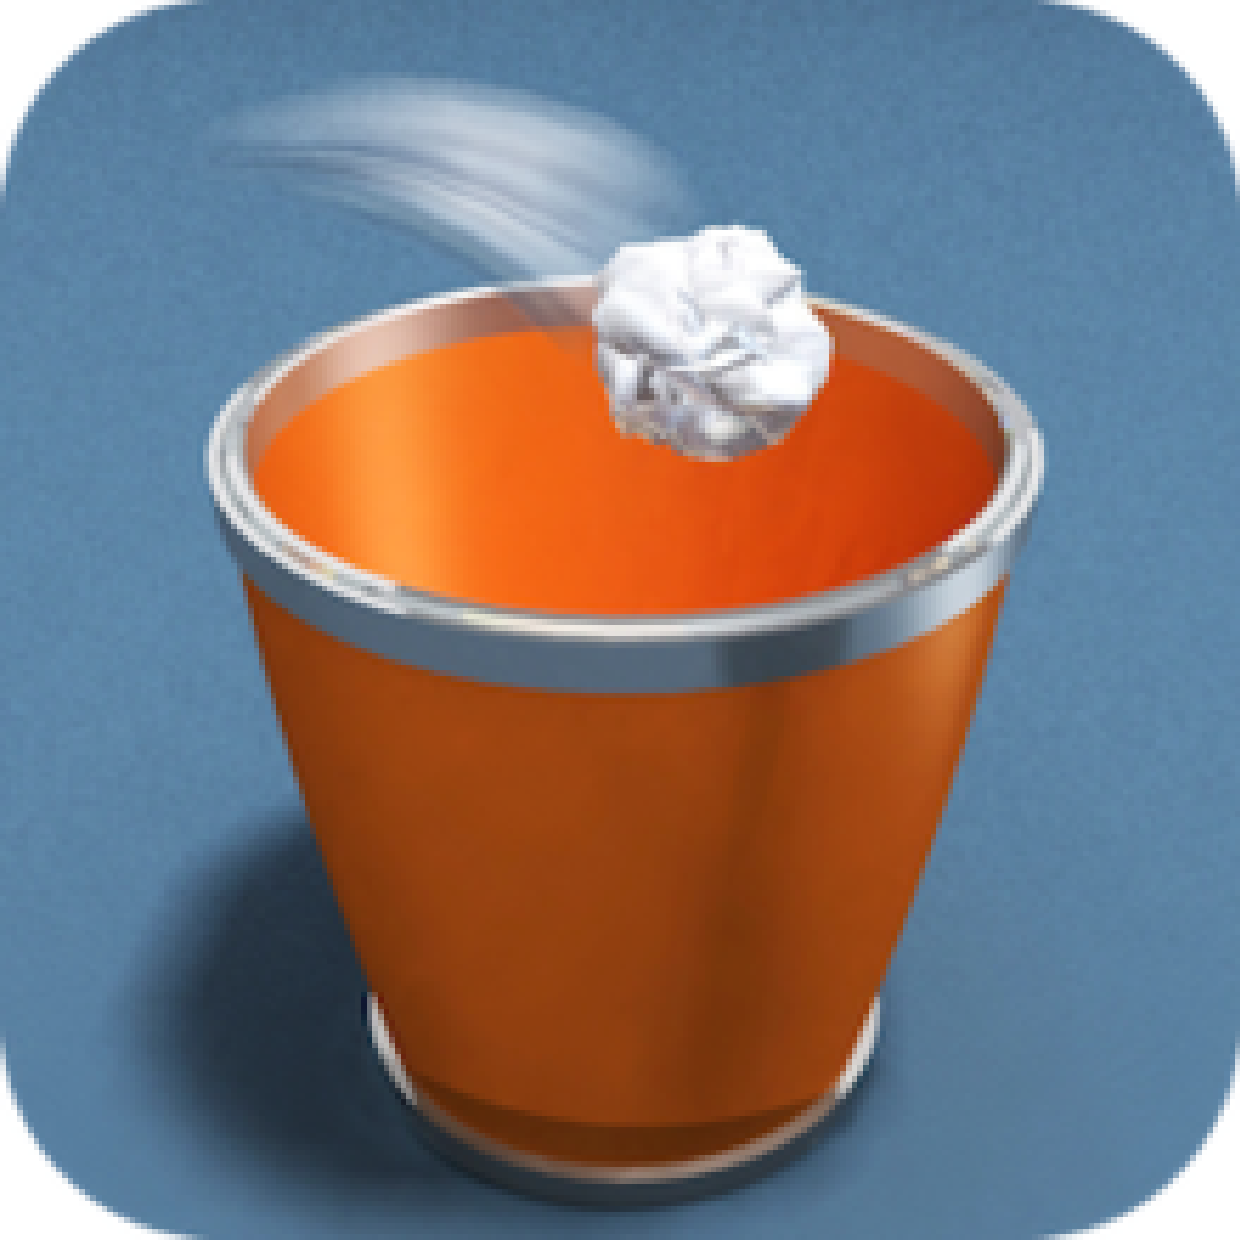
\includegraphics[width=0.4\paperwidth]{./Ressourcen/Figures/paper_toss_app.pdf}
	\end{textblock*}
	
	\begin{textblock*}{0.5\paperwidth}[1,1](\textwidth + \PraesentationSeitenrand, 18cm - \PraesentationSeitenrand)%
		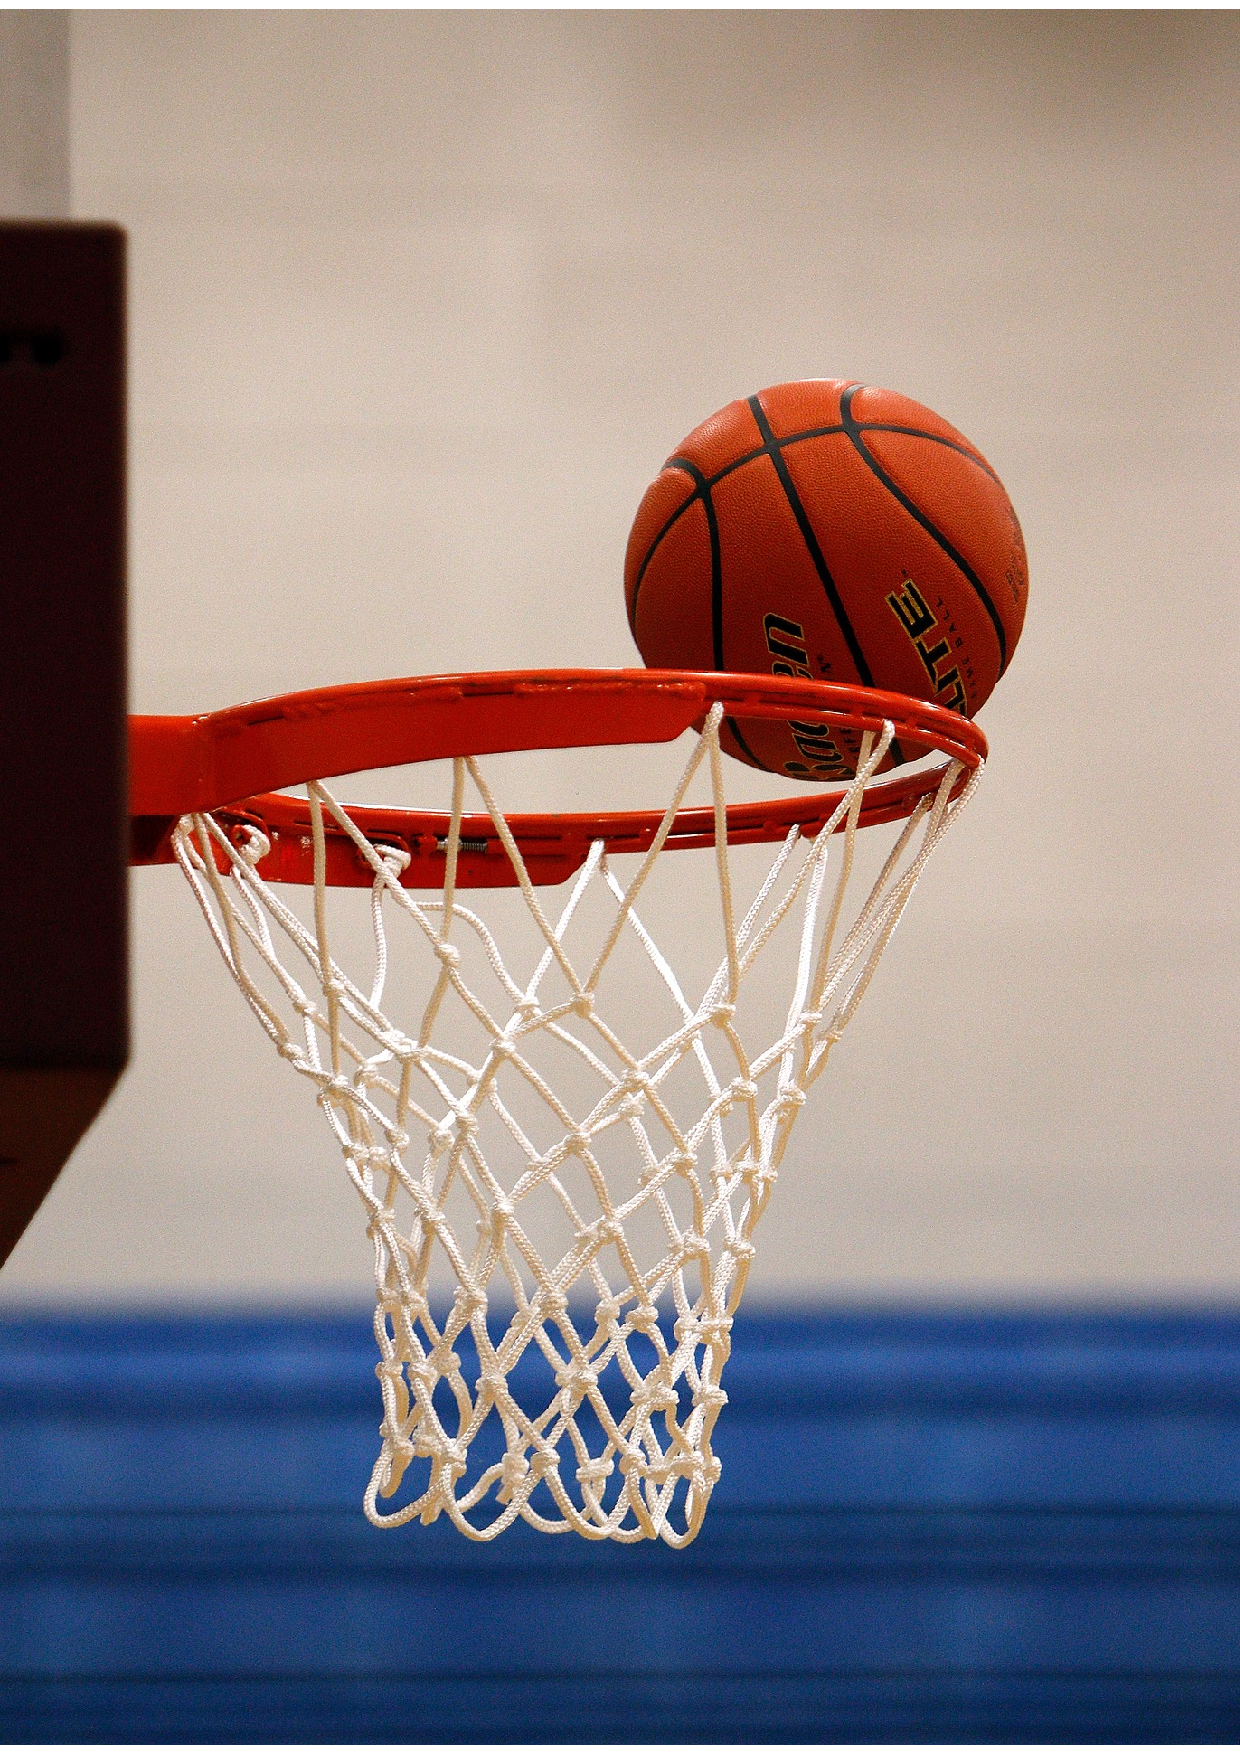
\includegraphics[width=0.4\paperwidth]{./Ressourcen/Figures/basketball.pdf}
	\end{textblock*}
	
\end{frame}
\clearpage

%%%%%%%%%%%%%%%%%%%%%%%%%%%%%%%%%%%%%%%%%%%%%%%%%%%%%%%%%%%%%%%%%%%%%%%%%%%%%%%%


% Seite 2

%%%%%%%%%%%%%%%%%%%%%%%%%%%%%%%%%%%%%%%%%%%%%%%%%%%%%%%%%%%%%%%%%%%%%%%%%%%%%%%%


\begin{frame}
	\frametitle{Outline}
	
	\vspace{1cm}
	\begin{PraesentationAufzaehlung}
		\item Motivation
		\item Reinforcement Learning
		\item Hindsight Experience Replay
		\item Methodology
		\item Experiment 1: FetchSlideball (Golf)
		\item Experiment 2: FetchToss
		\item Conclusion/Future Work
	\end{PraesentationAufzaehlung}
	
\end{frame}
\clearpage

%%%%%%%%%%%%%%%%%%%%%%%%%%%%%%%%%%%%%%%%%%%%%%%%%%%%%%%%%%%%%%%%%%%%%%%%%%%%%%%%



% Seite 3


%%%%%%%%%%%%%%%%%%%%%%%%%%%%%%%%%%%%%%%%%%%%%%%%%%%%%%%%%%%%%%%%%%%%%%%%%%%%%%%%

\begin{frame}
	\frametitle{Reinforcement Learning}	
	\vspace{1cm}

    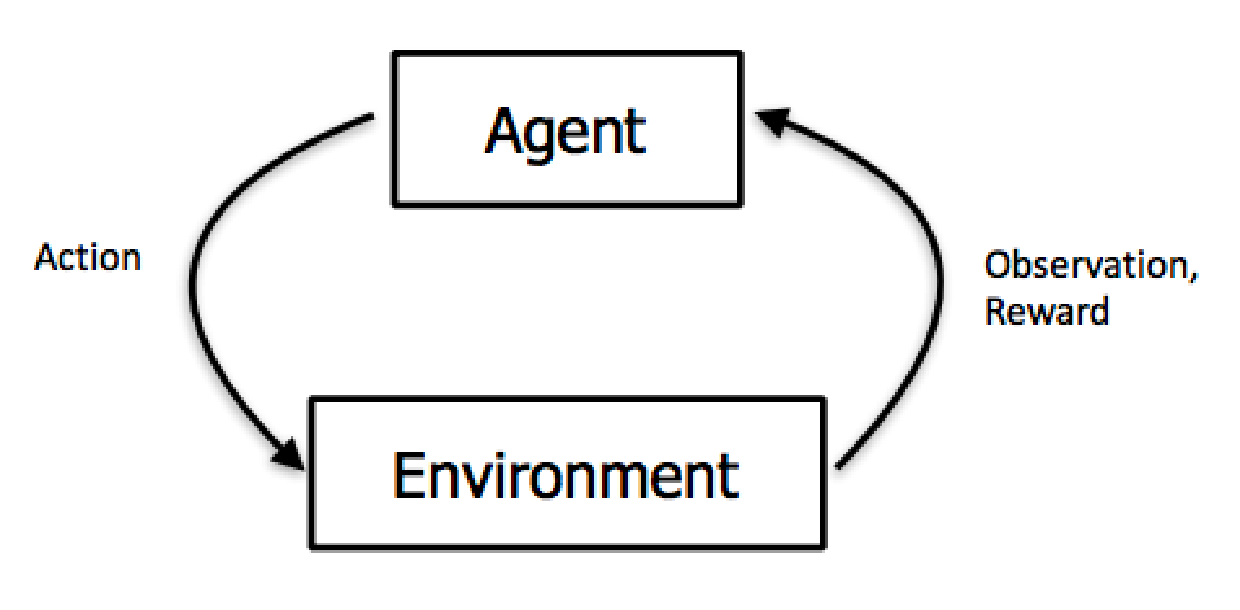
\includegraphics[width=\textwidth, height=.55\textheight]{./Ressourcen/Figures/reinforcementlearning.pdf}%

\end{frame}
\clearpage

%%%%%%%%%%%%%%%%%%%%%%%%%%%%%%%%%%%%%%%%%%%%%%%%%%%%%%%%%%%%%%%%%%%%%%%%%%%%%%%%


% Seite 4


%%%%%%%%%%%%%%%%%%%%%%%%%%%%%%%%%%%%%%%%%%%%%%%%%%%%%%%%%%%%%%%%%%%%%%%%%%%%%%%%

\begin{frame}
	\frametitle{Hindsight Experience Replay}	
	\vspace{1cm}
	
	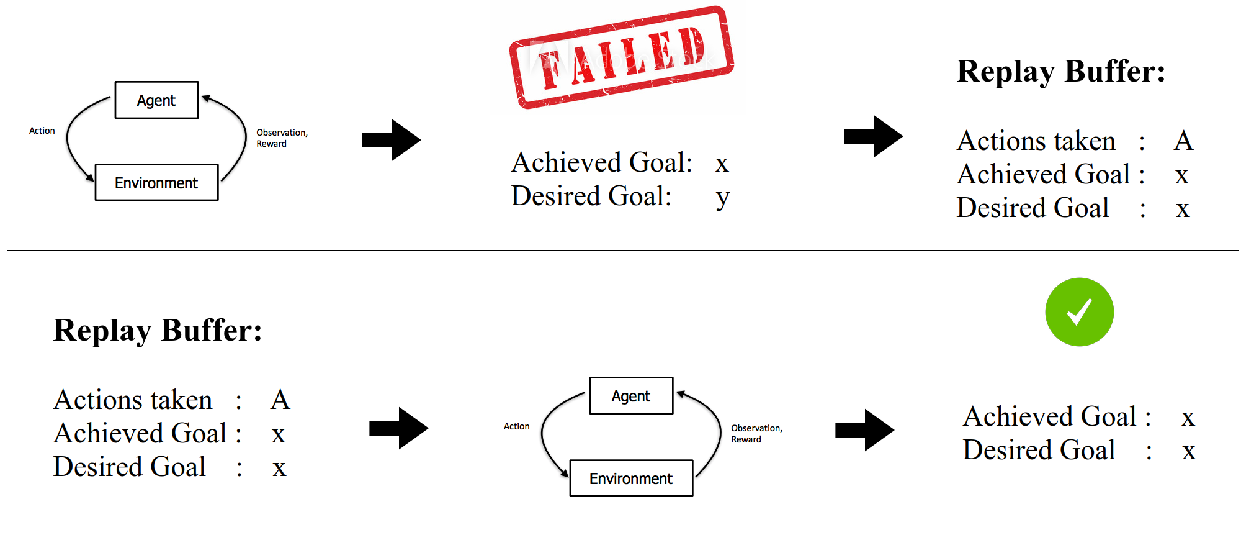
\includegraphics[width=\textwidth, height=.55\textheight]{./Ressourcen/Figures/her.pdf}%
	
\end{frame}
\clearpage

%%%%%%%%%%%%%%%%%%%%%%%%%%%%%%%%%%%%%%%%%%%%%%%%%%%%%%%%%%%%%%%%%%%%%%%%%%%%%%%%


% Seite 5


%%%%%%%%%%%%%%%%%%%%%%%%%%%%%%%%%%%%%%%%%%%%%%%%%%%%%%%%%%%%%%%%%%%%%%%%%%%%%%%%

\begin{frame}
	\frametitle{Methodology}	
	\vspace{1cm}
	
	\begin{PraesentationAufzaehlung}
		\item Run Benchmarks (by OpenAI)
		\item Test a simpler environment first (Golf/Slideball)
		\item Then create the tossing environment (Basketball)
		\item For both golf and toss: \\
		 - Compare using a ball \\
		 - Try different distance, height, weight etc.\\
	\end{PraesentationAufzaehlung}
	
\end{frame}
\clearpage

%%%%%%%%%%%%%%%%%%%%%%%%%%%%%%%%%%%%%%%%%%%%%%%%%%%%%%%%%%%%%%%%%%%%%%%%%%%%%%%%


% Seite 6


%%%%%%%%%%%%%%%%%%%%%%%%%%%%%%%%%%%%%%%%%%%%%%%%%%%%%%%%%%%%%%%%%%%%%%%%%%%%%%%%

\begin{frame}
	\frametitle{Benchmarks}	
	\vspace{1cm}

	%TODO video with all 4 ?
	
	
	\begin{textblock*}{0.4\paperwidth}[0,1](3cm, 10cm - \PraesentationSeitenrand)%
		FetchReach-v1
		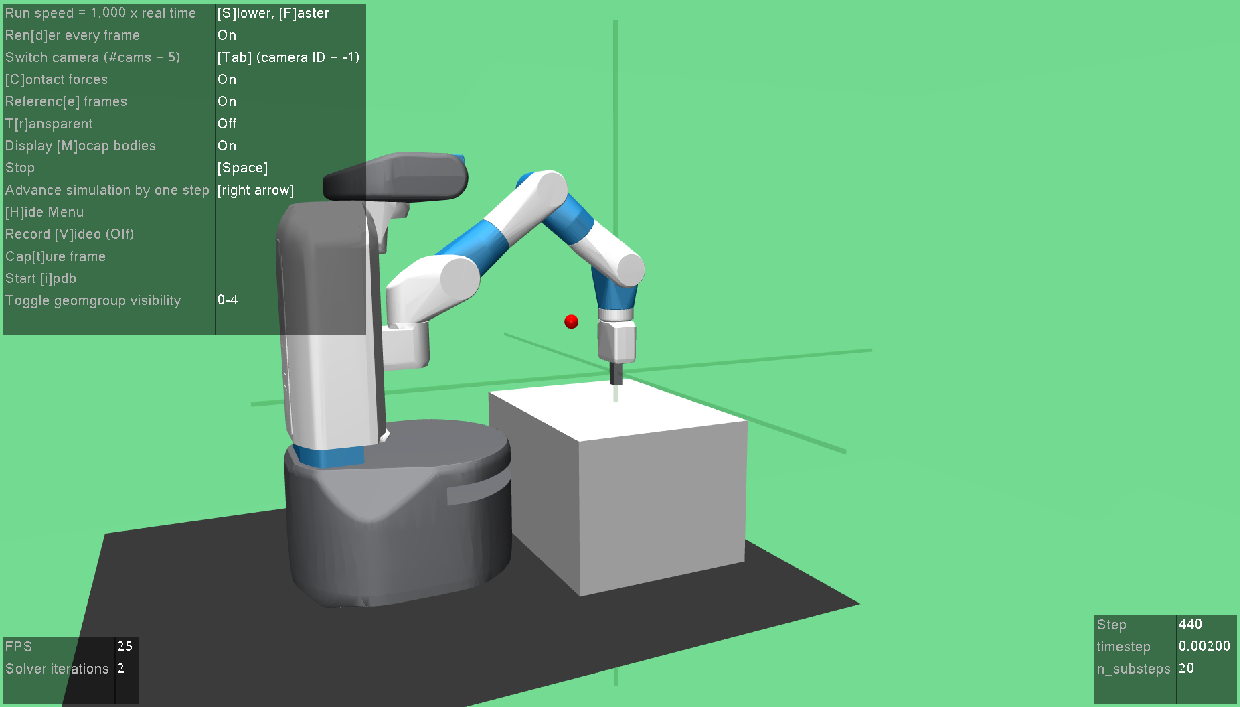
\includegraphics[width=0.3\paperwidth]{./Ressourcen/Figures/FetchReach-v1.pdf}
	\end{textblock*}
	
	\begin{textblock*}{0.4\paperwidth}[1,1](\textwidth + \PraesentationSeitenrand, 10cm - \PraesentationSeitenrand)%
		FetchPush-v1
		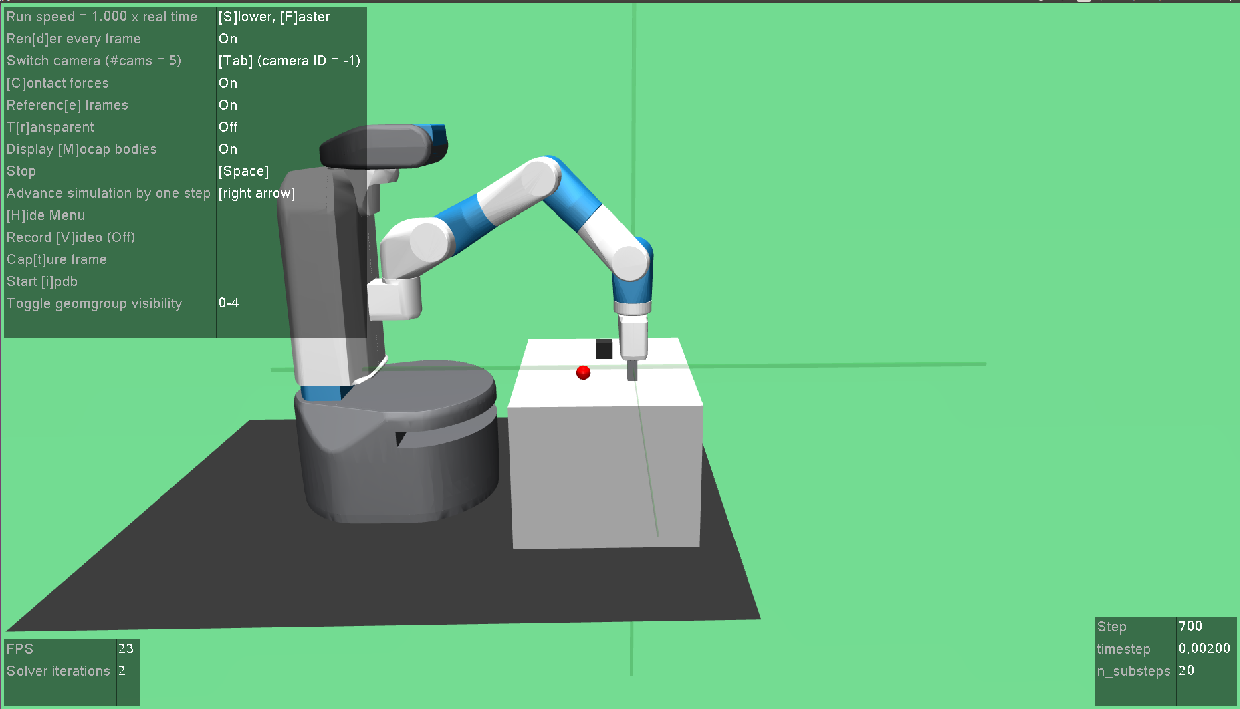
\includegraphics[width=0.3\paperwidth]{./Ressourcen/Figures/FetchPush-v1.pdf}
	\end{textblock*}
	
	\begin{textblock*}{0.4\paperwidth}[0,1](3cm, 17cm - \PraesentationSeitenrand)%
		FetchSlide-v1
		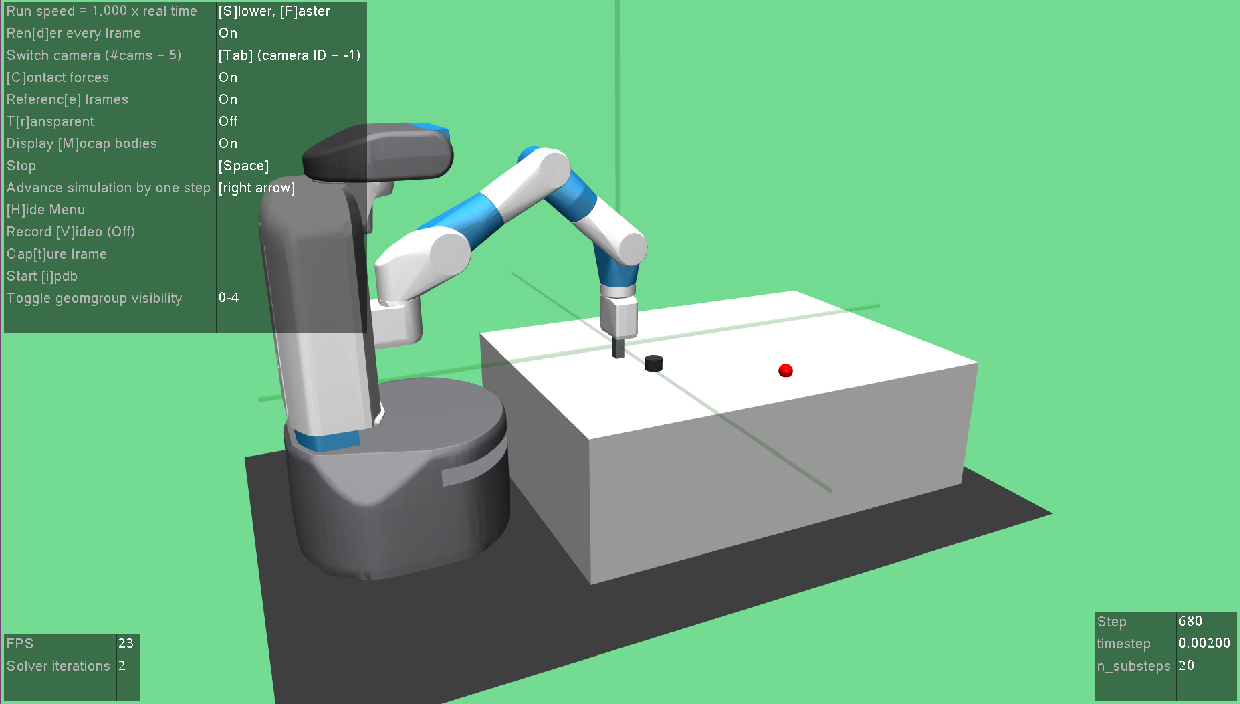
\includegraphics[width=0.3\paperwidth]{./Ressourcen/Figures/FetchSlide-v1.pdf}
	\end{textblock*}
	
	\begin{textblock*}{0.4\paperwidth}[1,1](\textwidth + \PraesentationSeitenrand, 17cm - \PraesentationSeitenrand)%
		FetchPickAndPlace-v1
		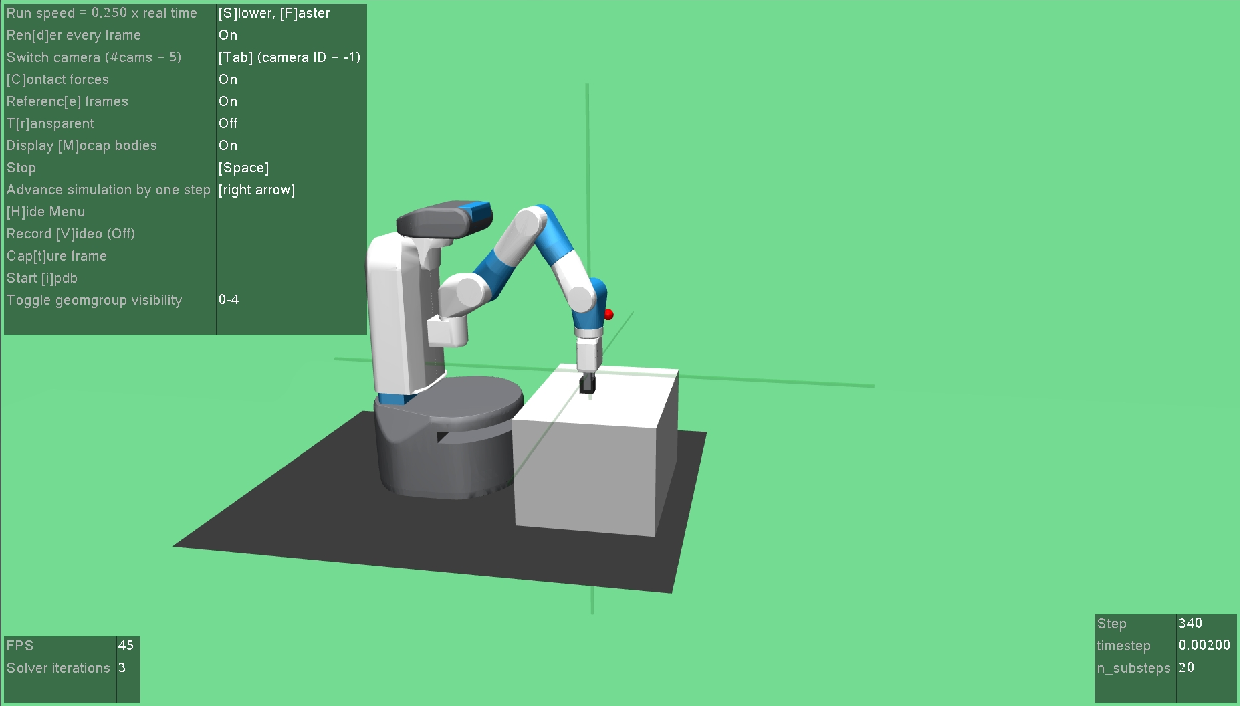
\includegraphics[width=0.3\paperwidth]{./Ressourcen/Figures/FetchPickAndPlace-v1.pdf}
	\end{textblock*}
	
	
	
\end{frame}
\clearpage

%%%%%%%%%%%%%%%%%%%%%%%%%%%%%%%%%%%%%%%%%%%%%%%%%%%%%%%%%%%%%%%%%%%%%%%%%%%%%%%%


% Seite 7

%%%%%%%%%%%%%%%%%%%%%%%%%%%%%%%%%%%%%%%%%%%%%%%%%%%%%%%%%%%%%%%%%%%%%%%%%%%%%%%%

\begin{frame}
	\frametitle{Benchmarks}	
	\vspace{1cm}
	
	
	\begin{textblock*}{0.5\paperwidth}[0,1](3cm, 11cm - \PraesentationSeitenrand)%
		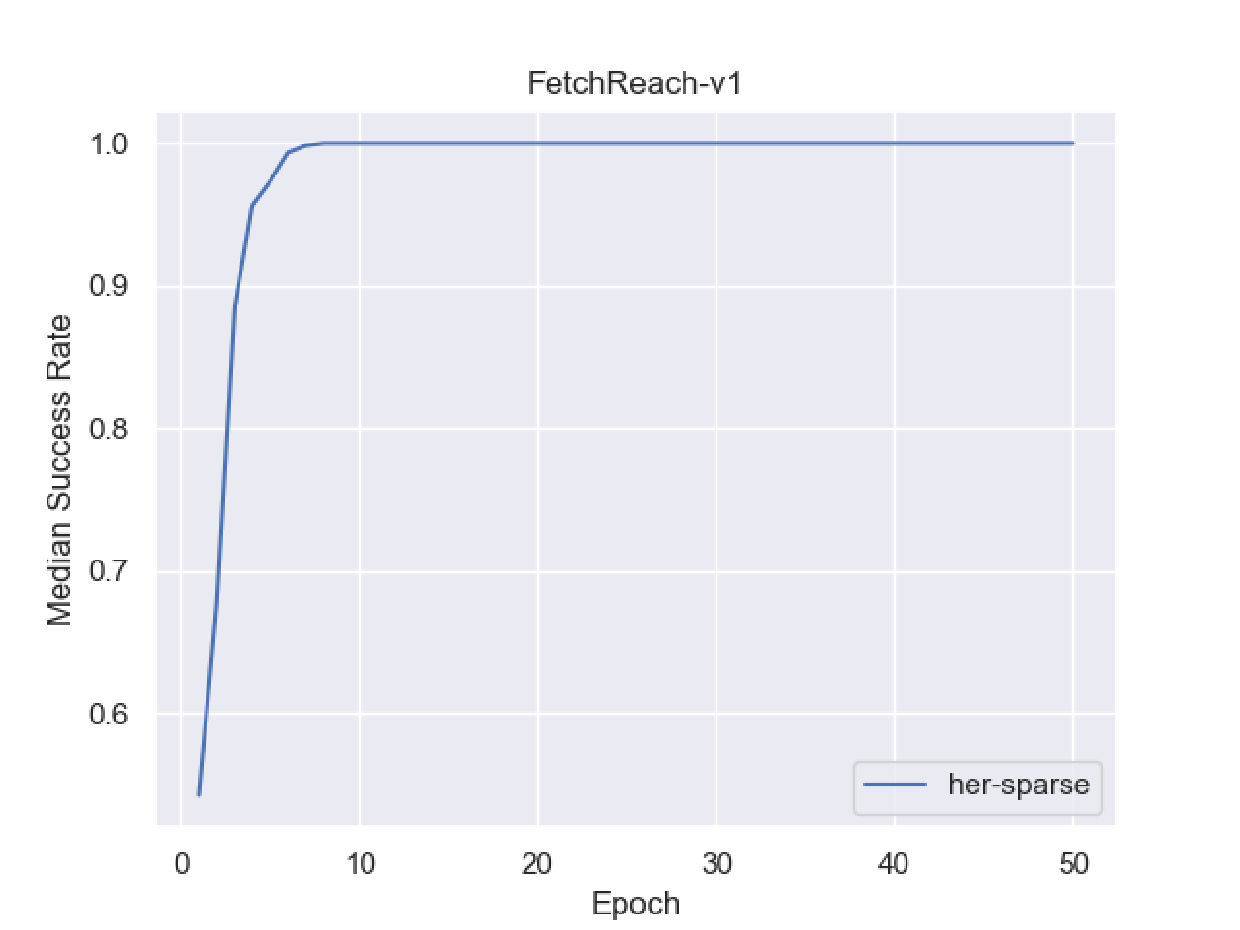
\includegraphics[width=0.3\paperwidth]{./Ressourcen/Figures/fig_FetchReach-v1.pdf}
	\end{textblock*}
	
	\begin{textblock*}{0.5\paperwidth}[1,1](\textwidth + 2cm + \PraesentationSeitenrand, 11cm - \PraesentationSeitenrand)%
		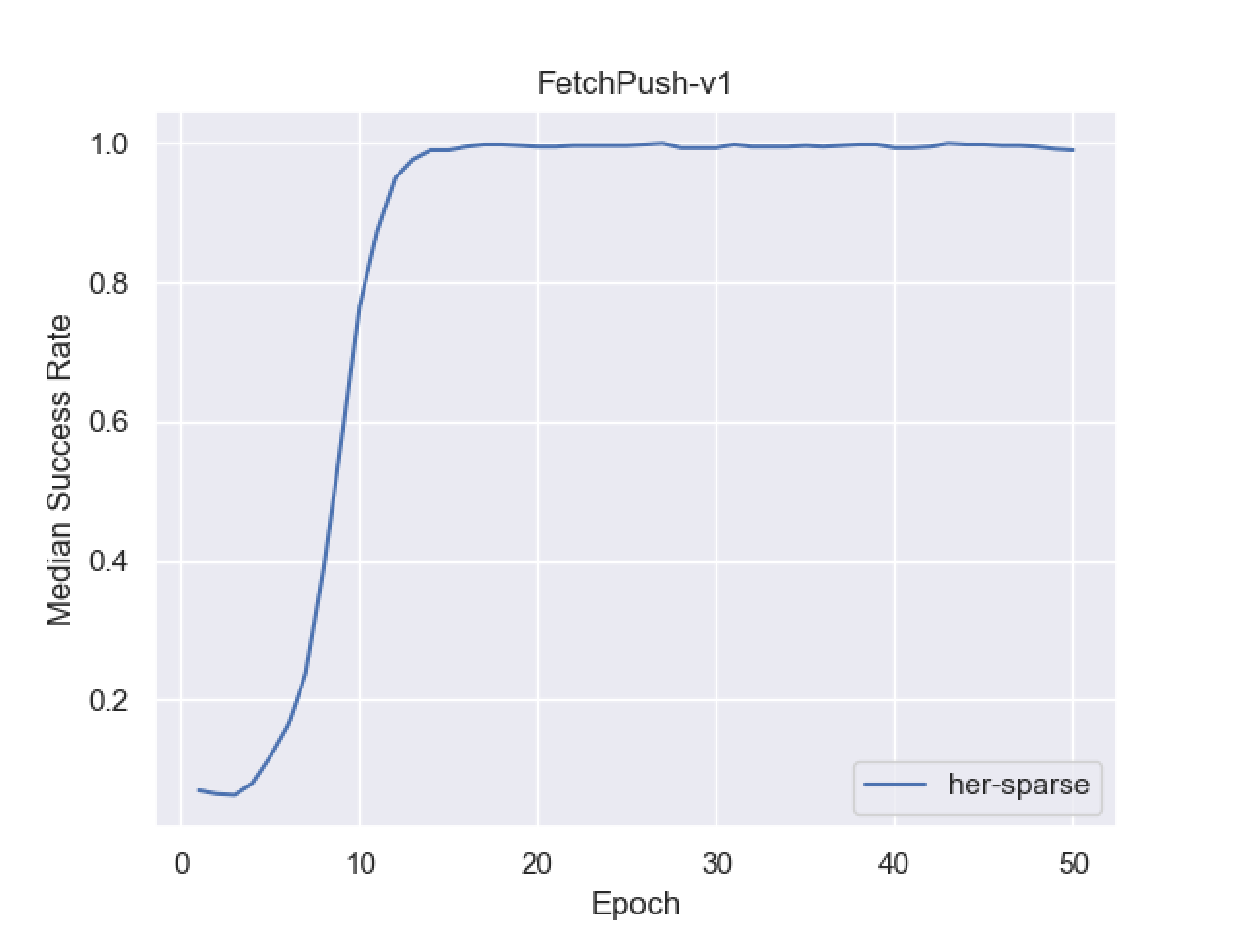
\includegraphics[width=0.3\paperwidth]{./Ressourcen/Figures/fig_FetchPush-v1.pdf}
	\end{textblock*}
	
	\begin{textblock*}{0.5\paperwidth}[0,1](3cm, 17cm - \PraesentationSeitenrand)%
		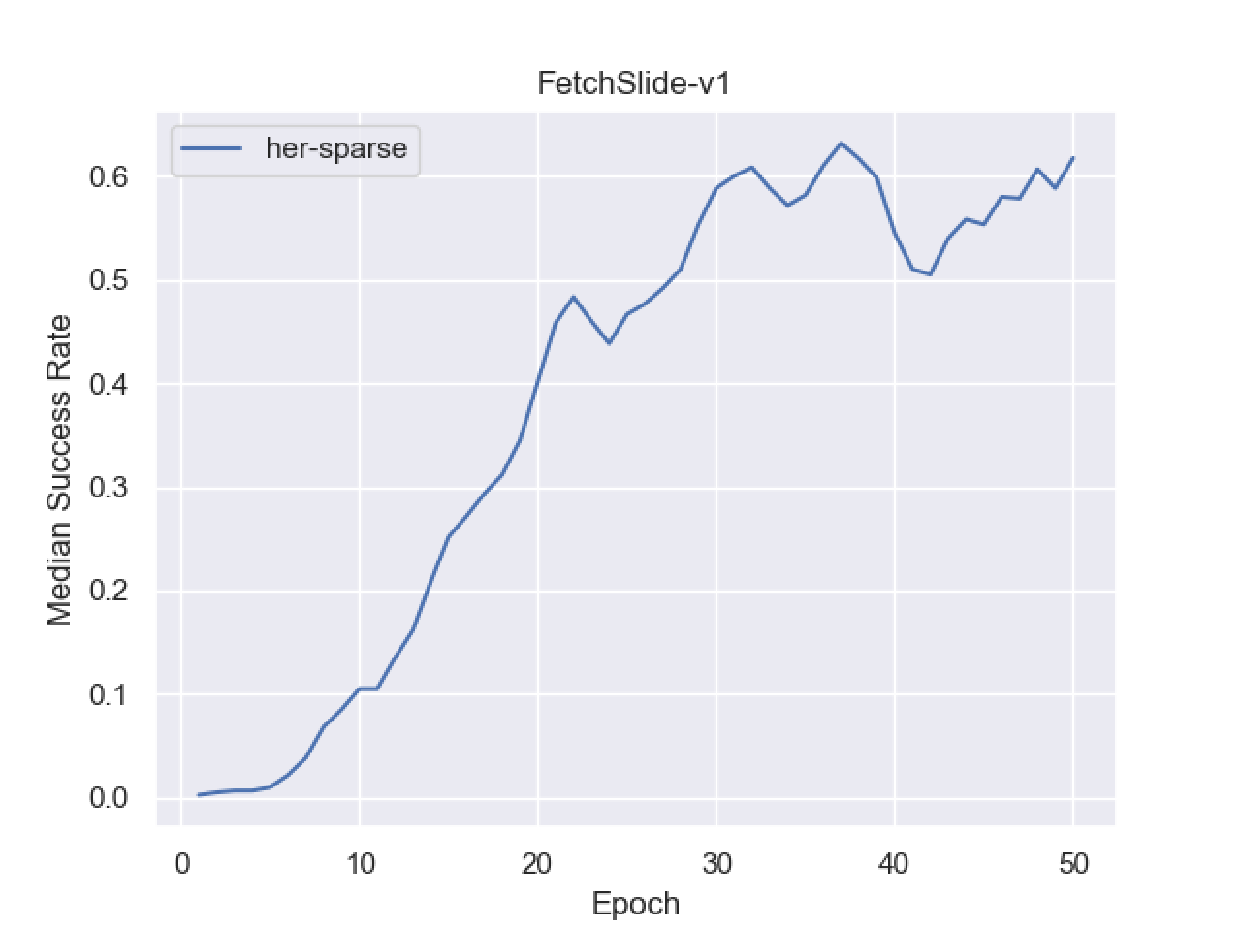
\includegraphics[width=0.3\paperwidth]{./Ressourcen/Figures/fig_FetchSlide-v1.pdf}
	\end{textblock*}
	
	\begin{textblock*}{0.5\paperwidth}[1,1](\textwidth + 2cm + \PraesentationSeitenrand, 17cm - \PraesentationSeitenrand)%
		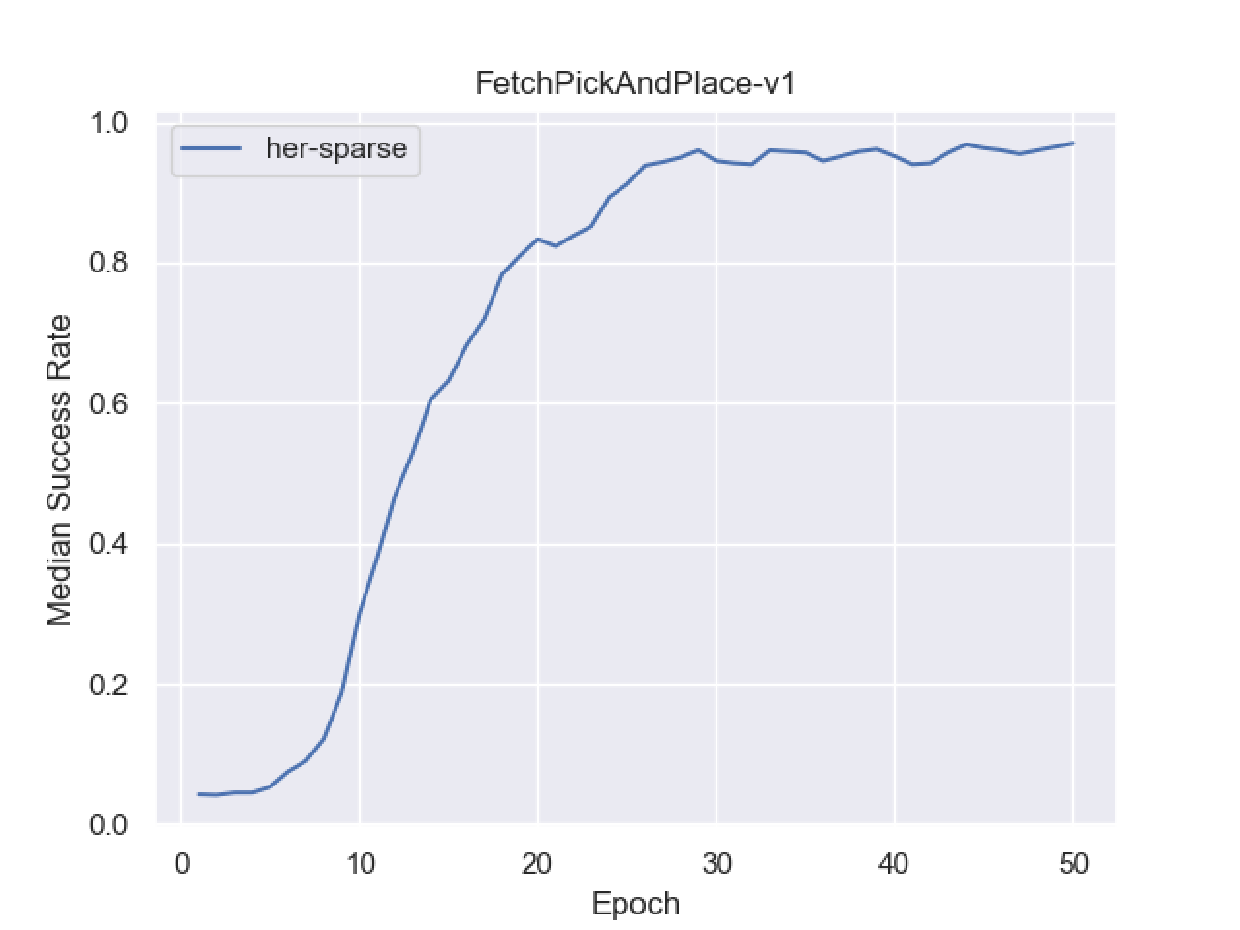
\includegraphics[width=0.3\paperwidth]{./Ressourcen/Figures/fig_FetchPickAndPlace-v1.pdf}
	\end{textblock*}
	
	
	
\end{frame}
\clearpage

%%%%%%%%%%%%%%%%%%%%%%%%%%%%%%%%%%%%%%%%%%%%%%%%%%%%%%%%%%%%%%%%%%%%%%%%%%%%%%%%


% Seite 8


%%%%%%%%%%%%%%%%%%%%%%%%%%%%%%%%%%%%%%%%%%%%%%%%%%%%%%%%%%%%%%%%%%%%%%%%%%%%%%%%

\begin{frame}
	\frametitle{FetchSlideball}	
	\vspace{1cm}
	
	%%Extending FetchSlide
	%%Explain Idea etc.. Why did I do this ? -> to test longer distance for tossing later. simpler than tossing
	FetchSlideball-v3
	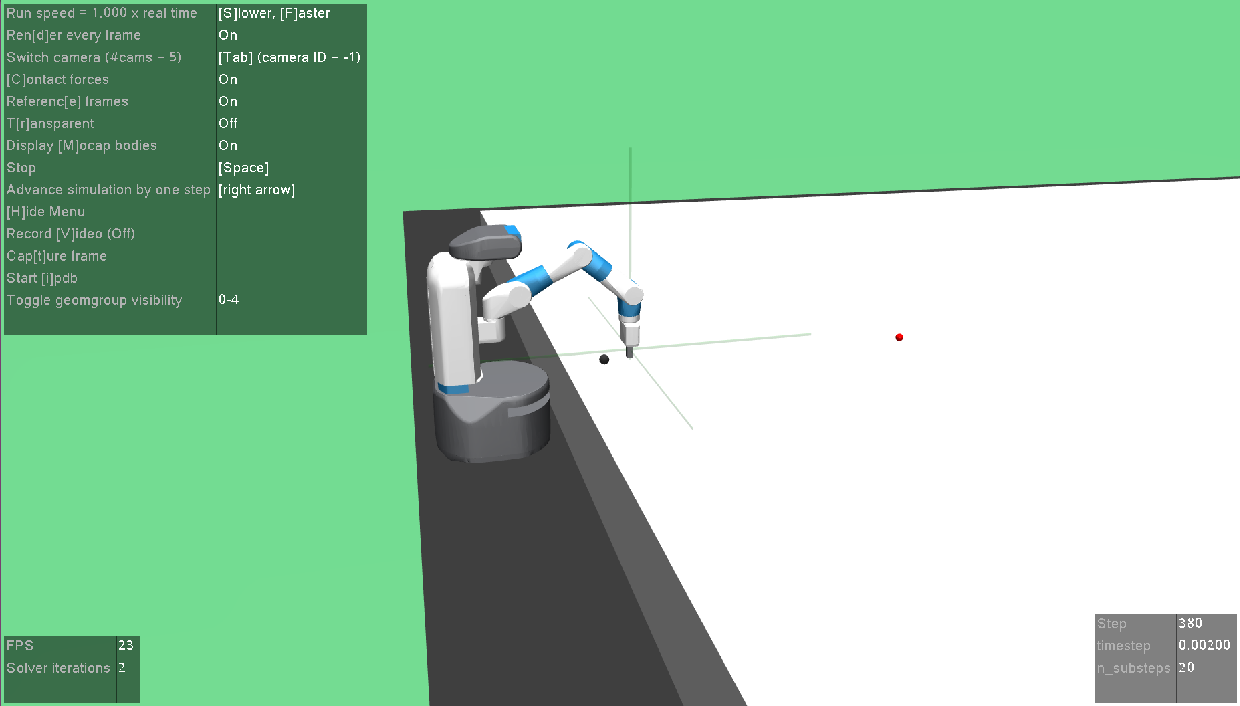
\includegraphics[width=\textwidth, height=.55\textheight]{./Ressourcen/Figures/FetchSlideball-v3.pdf}
	
	%Goal: bigger distance
	
\end{frame}
\clearpage

%%%%%%%%%%%%%%%%%%%%%%%%%%%%%%%%%%%%%%%%%%%%%%%%%%%%%%%%%%%%%%%%%%%%%%%%%%%%%%%%




% Seite 9


%%%%%%%%%%%%%%%%%%%%%%%%%%%%%%%%%%%%%%%%%%%%%%%%%%%%%%%%%%%%%%%%%%%%%%%%%%%%%%%%

\begin{frame}
	\frametitle{FetchSlideball Version 1}	
	\vspace{1cm}
	
	Same as FetchSlide-v1, but with a ball
	
    %Bild FetchSlide-v1
    
    \begin{textblock*}{0.5\paperwidth}[1,1](\textwidth + \PraesentationSeitenrand, 14cm - \PraesentationSeitenrand)%
    	FetchSlideball-v1 (ball)
    	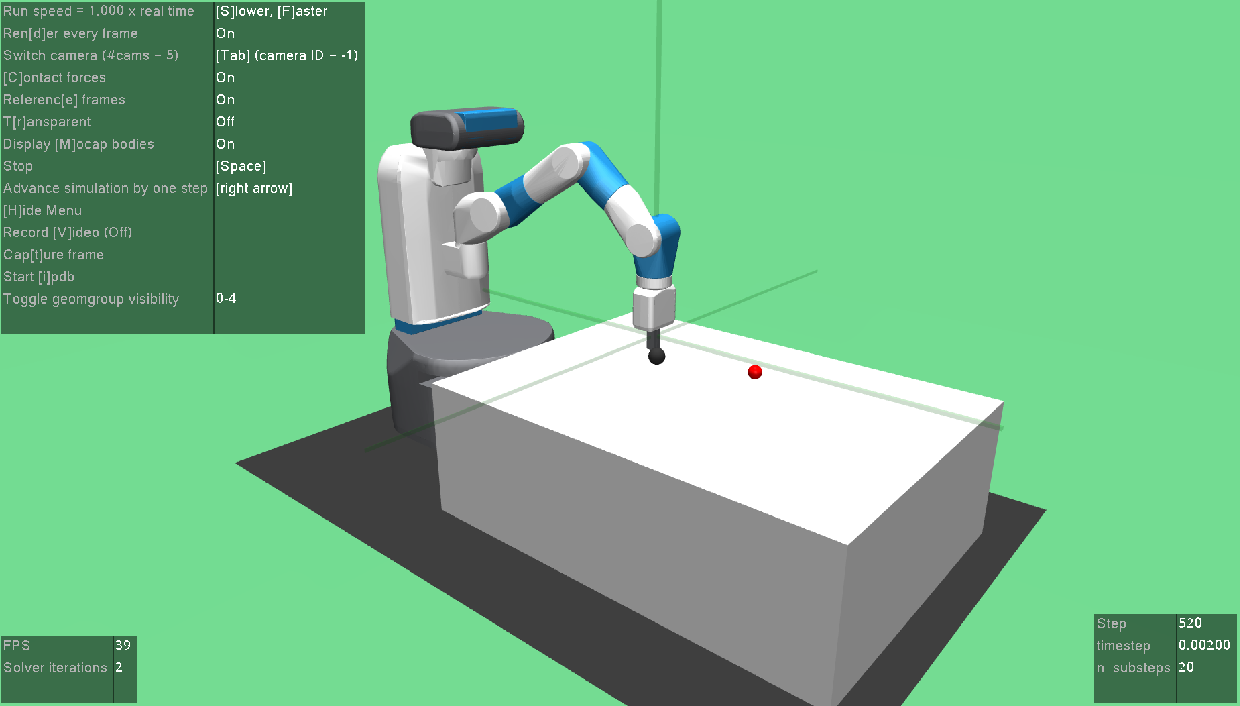
\includegraphics[width=0.4\paperwidth]{./Ressourcen/Figures/FetchSlideball-v1.pdf}
    \end{textblock*}
    
    	
	%Bild FetchSlideball-v1
	
    \begin{textblock*}{0.4\paperwidth}[0,1](0cm, 14cm - \PraesentationSeitenrand)%
    	FetchSlide-v1 (cylinder)
        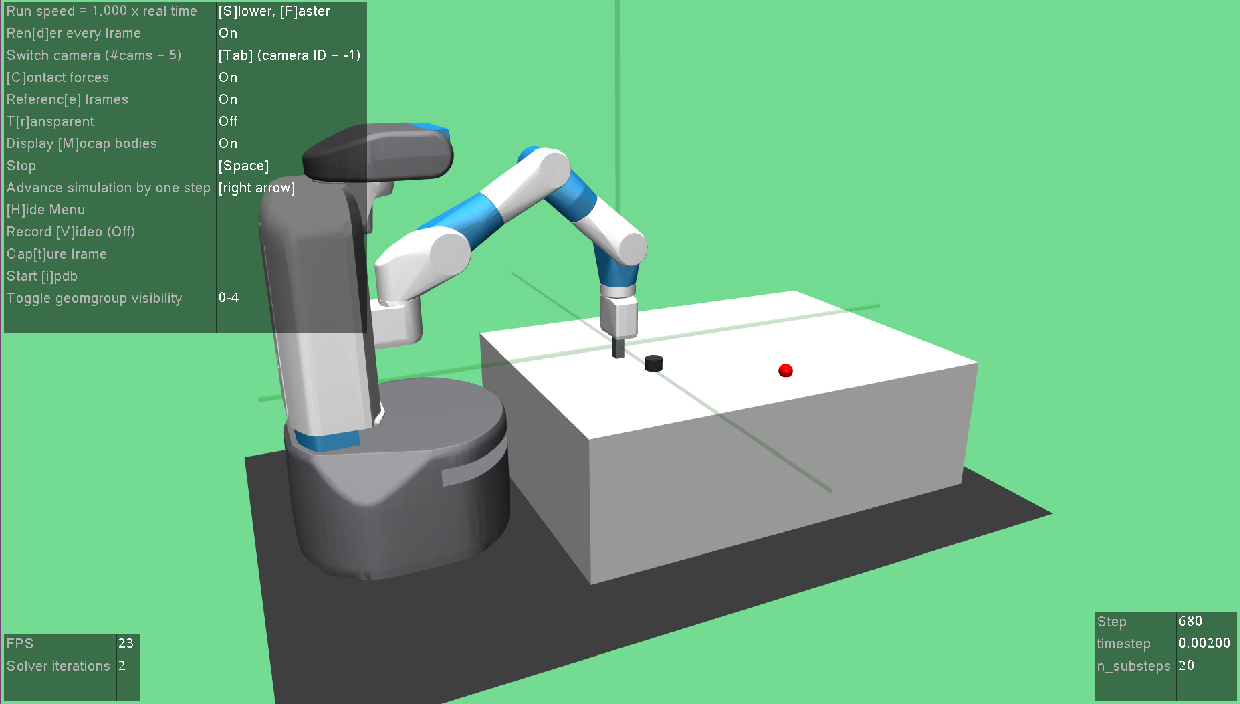
\includegraphics[width=0.4\paperwidth]{./Ressourcen/Figures/FetchSlide-v1.pdf}
    \end{textblock*}
    

	
	
\end{frame}
\clearpage

%%%%%%%%%%%%%%%%%%%%%%%%%%%%%%%%%%%%%%%%%%%%%%%%%%%%%%%%%%%%%%%%%%%%%%%%%%%%%%%%



% Seite 10


%%%%%%%%%%%%%%%%%%%%%%%%%%%%%%%%%%%%%%%%%%%%%%%%%%%%%%%%%%%%%%%%%%%%%%%%%%%%%%%%

\begin{frame}
	\frametitle{FetchSlideball Version 1}	
	\vspace{1cm}
	

		%Bild env
		\begin{textblock*}{0.4\paperwidth}[0,1](0cm, 13cm - \PraesentationSeitenrand)%
			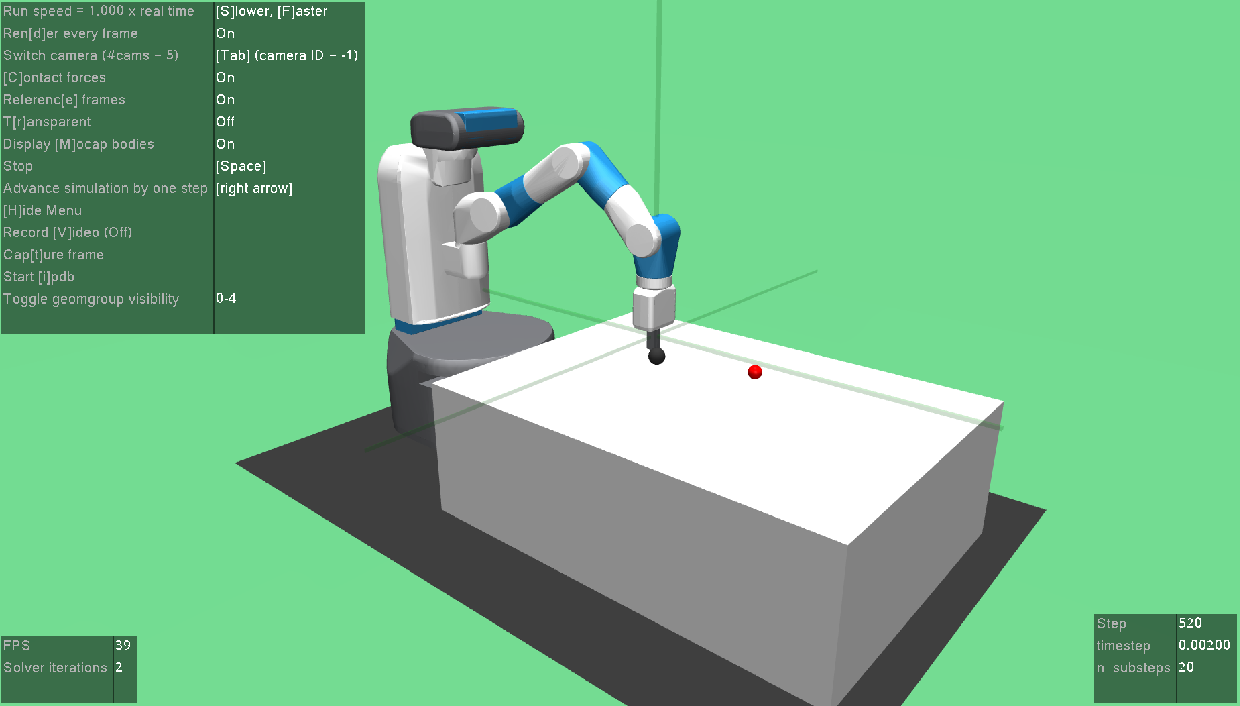
\includegraphics[width=0.4\paperwidth]{./Ressourcen/Figures/FetchSlideball-v1.pdf}
		\end{textblock*}
		
		%Bild FetchSlide-v1 vs FetchSlideball-v1
		\begin{textblock*}{0.5\paperwidth}[1,1](\textwidth + \PraesentationSeitenrand, 15cm - \PraesentationSeitenrand)%
			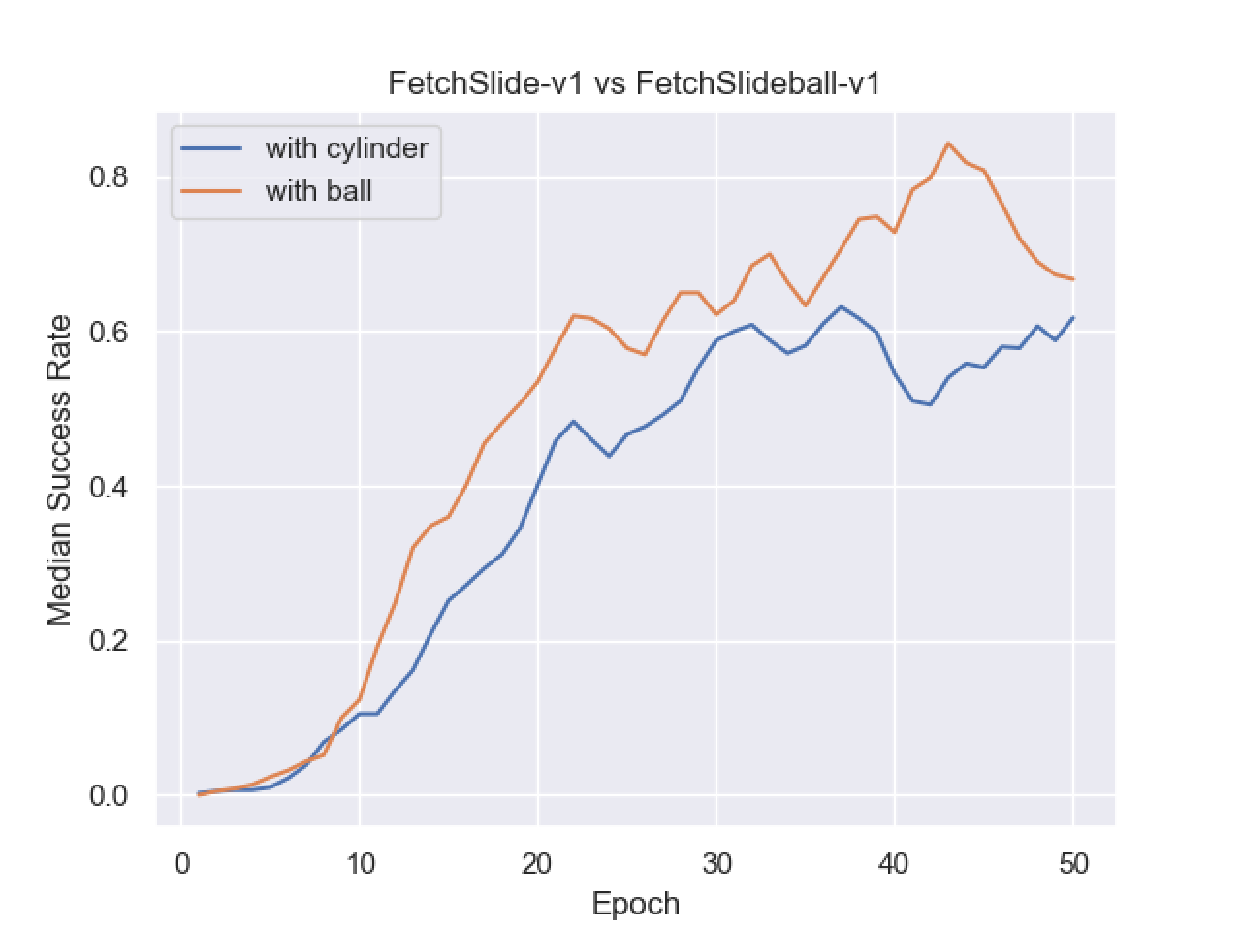
\includegraphics[width=0.5\paperwidth]{./Ressourcen/Figures/fig_FetchSlide-v1_vs_FetchSlideball-v1.pdf}
		\end{textblock*}
	
	
\end{frame}
\clearpage

%%%%%%%%%%%%%%%%%%%%%%%%%%%%%%%%%%%%%%%%%%%%%%%%%%%%%%%%%%%%%%%%%%%%%%%%%%%%%%%%




% Seite 10


%%%%%%%%%%%%%%%%%%%%%%%%%%%%%%%%%%%%%%%%%%%%%%%%%%%%%%%%%%%%%%%%%%%%%%%%%%%%%%%%

\begin{frame}
	\frametitle{FetchSlideball Version 2}	
	\vspace{1cm}
	Doubled the goal distance
	
	%Bild env
	
    \begin{textblock*}{0.4\paperwidth}[0,1](0cm, 15cm - \PraesentationSeitenrand)%
        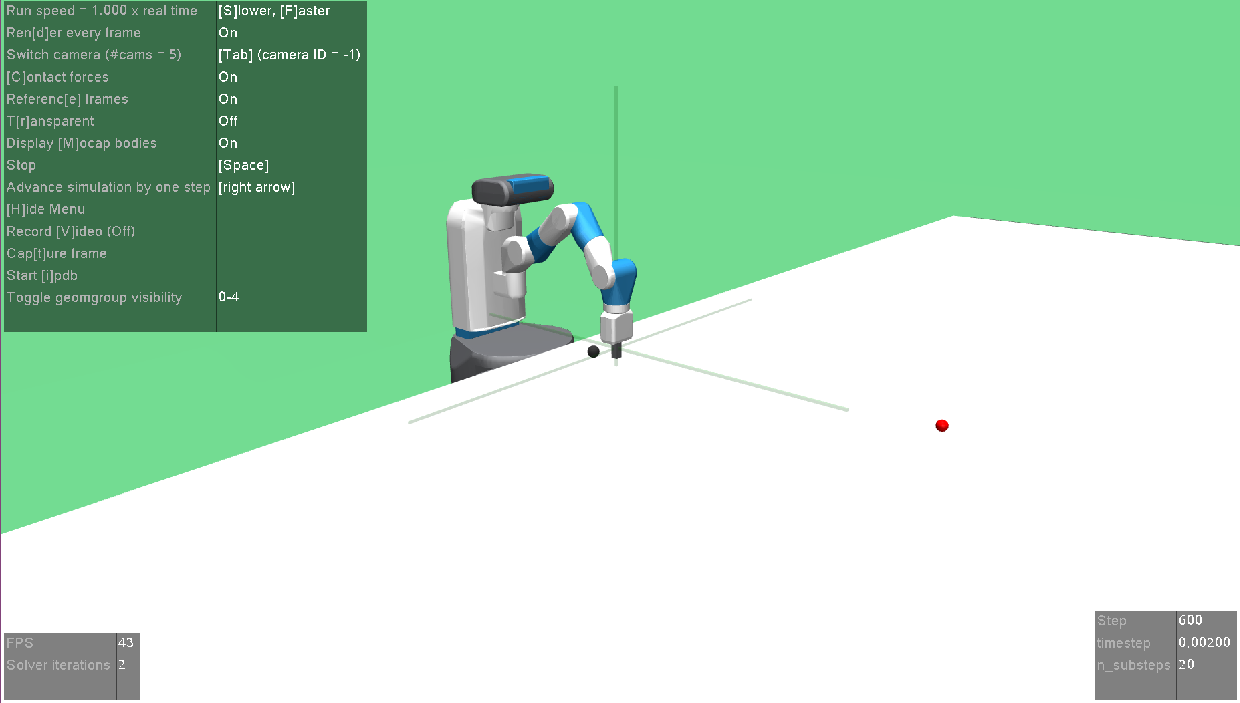
\includegraphics[width=0.4\paperwidth]{./Ressourcen/Figures/FetchSlideball-v2.pdf}
        
        Problem: Arm not strong enough too push it far enough -> decrease friction
    \end{textblock*}
    
    %Bild Success Rate
    
    \begin{textblock*}{0.5\paperwidth}[1,1](\textwidth + \PraesentationSeitenrand, 15cm - \PraesentationSeitenrand)%
    	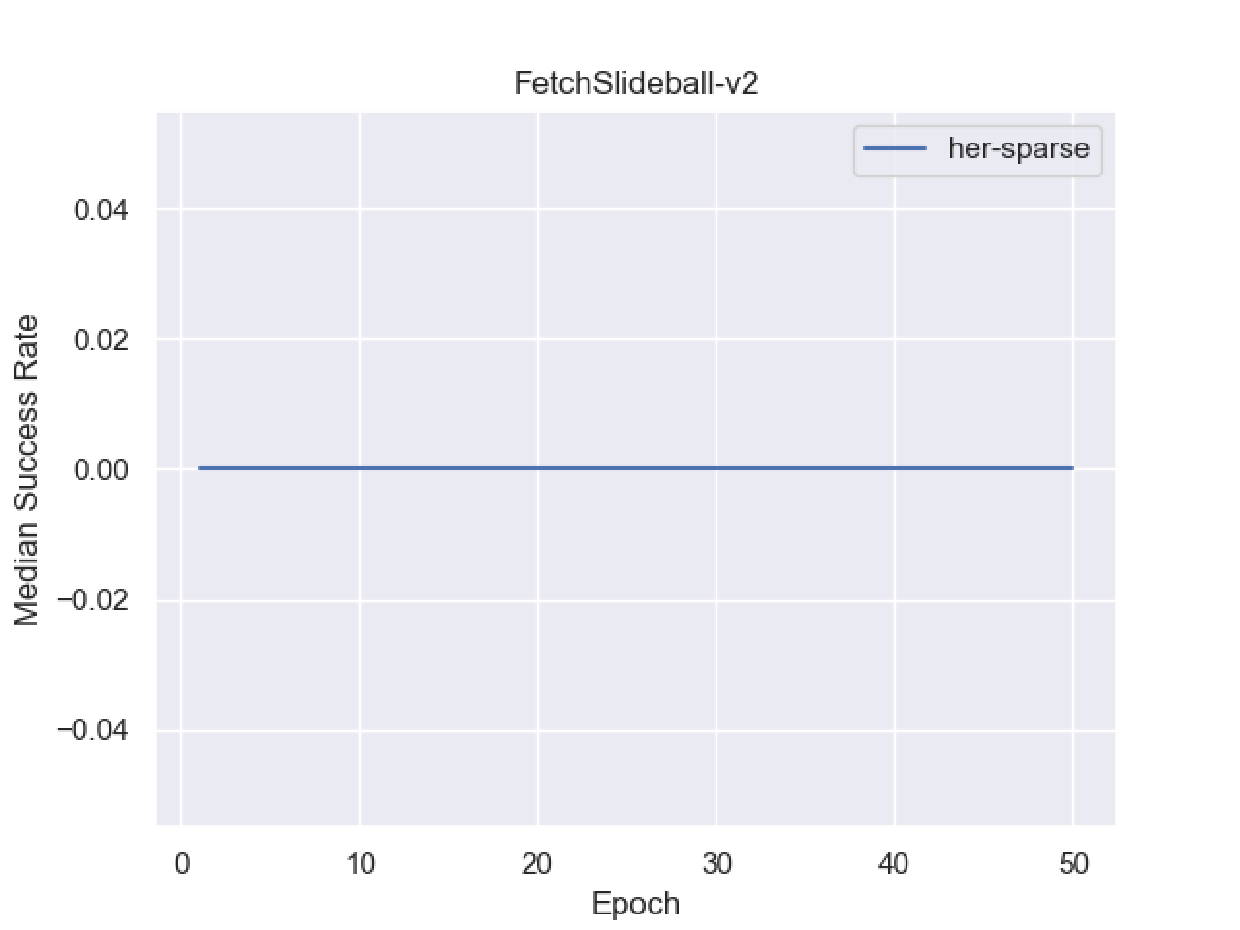
\includegraphics[width=0.5\paperwidth]{./Ressourcen/Figures/fig_FetchSlideball-v2.pdf}
    \end{textblock*}
	
	
	
	
\end{frame}
\clearpage

%%%%%%%%%%%%%%%%%%%%%%%%%%%%%%%%%%%%%%%%%%%%%%%%%%%%%%%%%%%%%%%%%%%%%%%%%%%%%%%%




% Seite 11


%%%%%%%%%%%%%%%%%%%%%%%%%%%%%%%%%%%%%%%%%%%%%%%%%%%%%%%%%%%%%%%%%%%%%%%%%%%%%%%%

\begin{frame}
	\frametitle{FetchSlideball with lower friction}	
	\vspace{1cm}
	
	%Bild env
	\begin{textblock*}{0.4\paperwidth}[0,1](0cm, 14cm - \PraesentationSeitenrand)%
		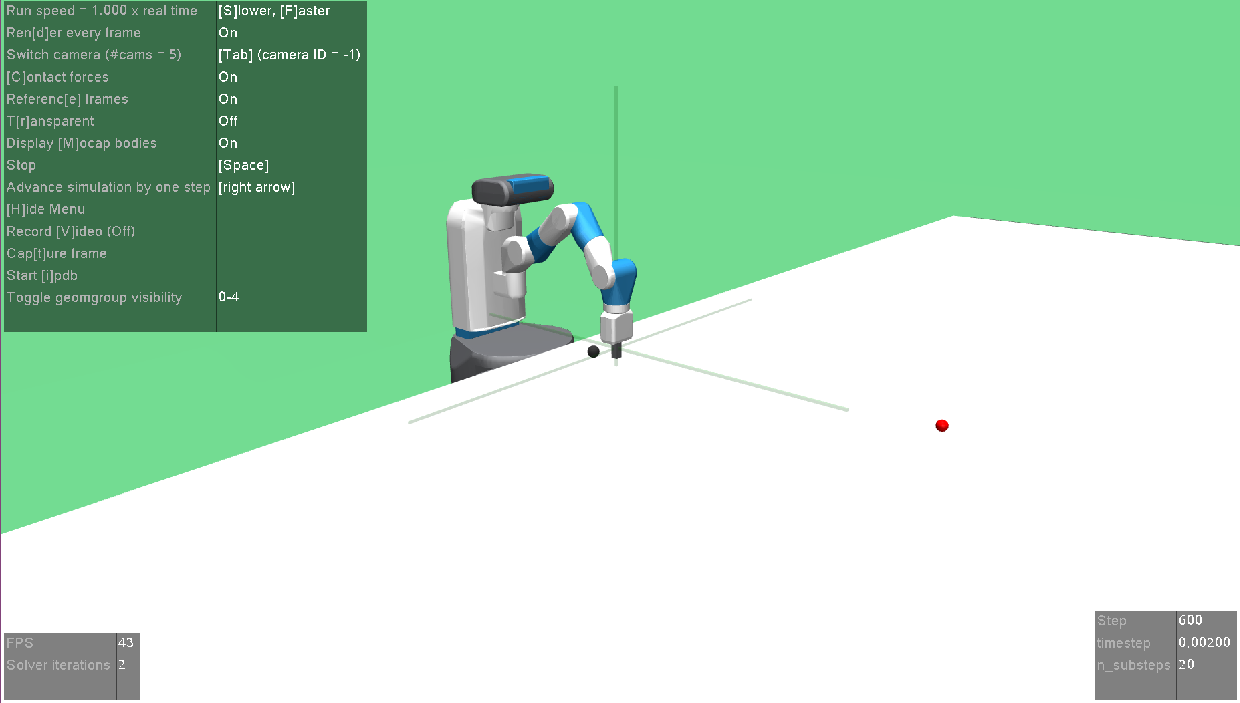
\includegraphics[width=0.4\paperwidth]{./Ressourcen/Figures/FetchSlideball-v2.pdf}
		
		-> learns direction but can't control distance 
	\end{textblock*}
	
	%Bild Success Rate
	\begin{textblock*}{0.5\paperwidth}[1,1](\textwidth + \PraesentationSeitenrand, 15cm - \PraesentationSeitenrand)%
		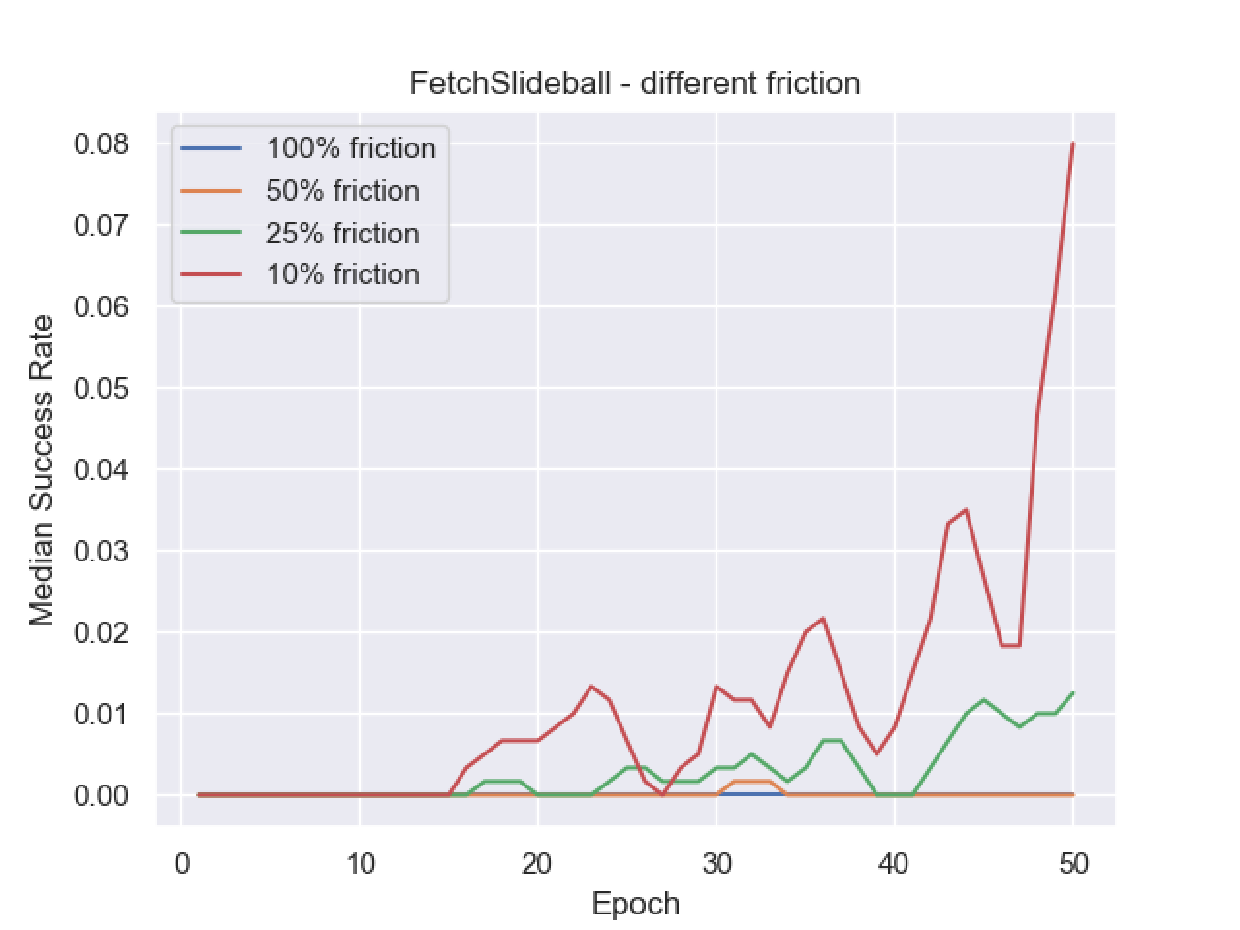
\includegraphics[width=0.5\paperwidth]{./Ressourcen/Figures/fig_FetchSlideball_friction.pdf}
	\end{textblock*}
	

	

	
\end{frame}
\clearpage

%%%%%%%%%%%%%%%%%%%%%%%%%%%%%%%%%%%%%%%%%%%%%%%%%%%%%%%%%%%%%%%%%%%%%%%%%%%%%%%%


% Seite 11.5

%%%%%%%%%%%%%%%%%%%%%%%%%%%%%%%%%%%%%%%%%%%%%%%%%%%%%%%%%%%%%%%%%%%%%%%%%%%%%%%%

\begin{frame}
	\frametitle{FetchSlideball with lower friction - 		\textbf{Slideball-v3 Video}}	
	\vspace{1cm}
	
	%Bild env
	\begin{textblock*}{0.4\paperwidth}[0,1](0cm, 14cm - \PraesentationSeitenrand)%
		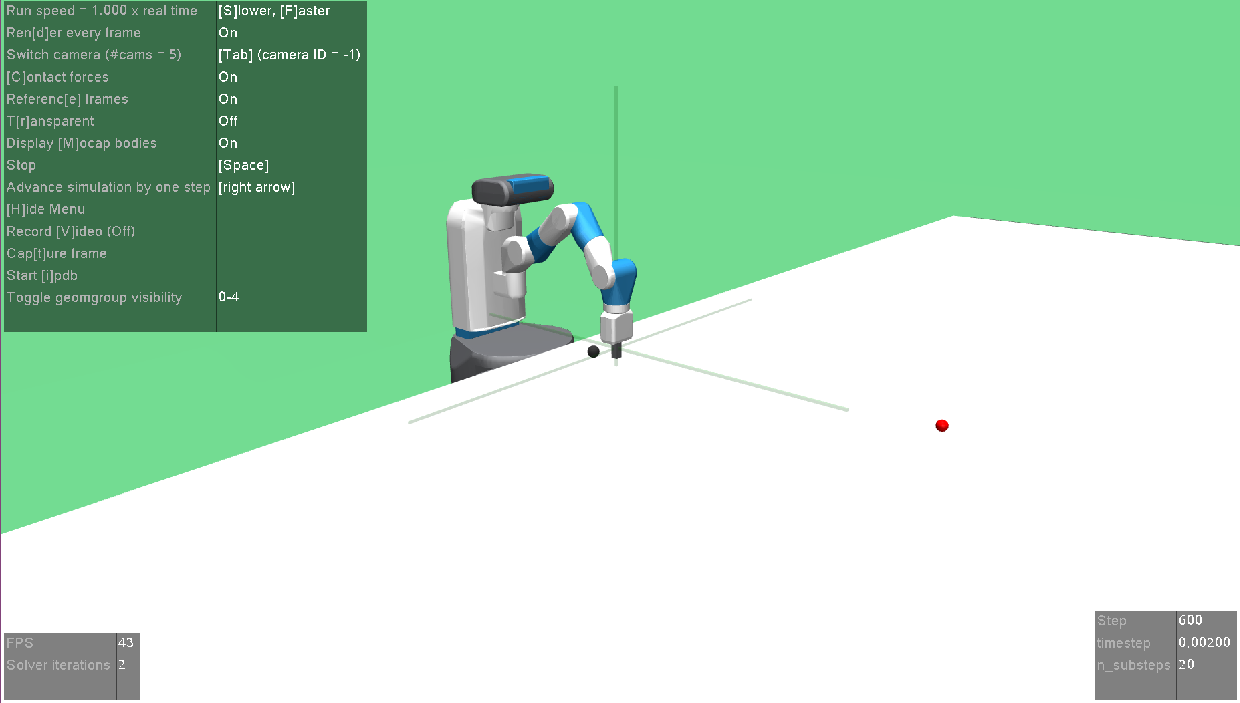
\includegraphics[width=0.4\paperwidth]{./Ressourcen/Figures/FetchSlideball-v2.pdf}
		
		-> learns direction but can't control distance 
	\end{textblock*}
	
	%Bild Success Rate
	\begin{textblock*}{0.5\paperwidth}[1,1](\textwidth + \PraesentationSeitenrand, 15cm - \PraesentationSeitenrand)%
		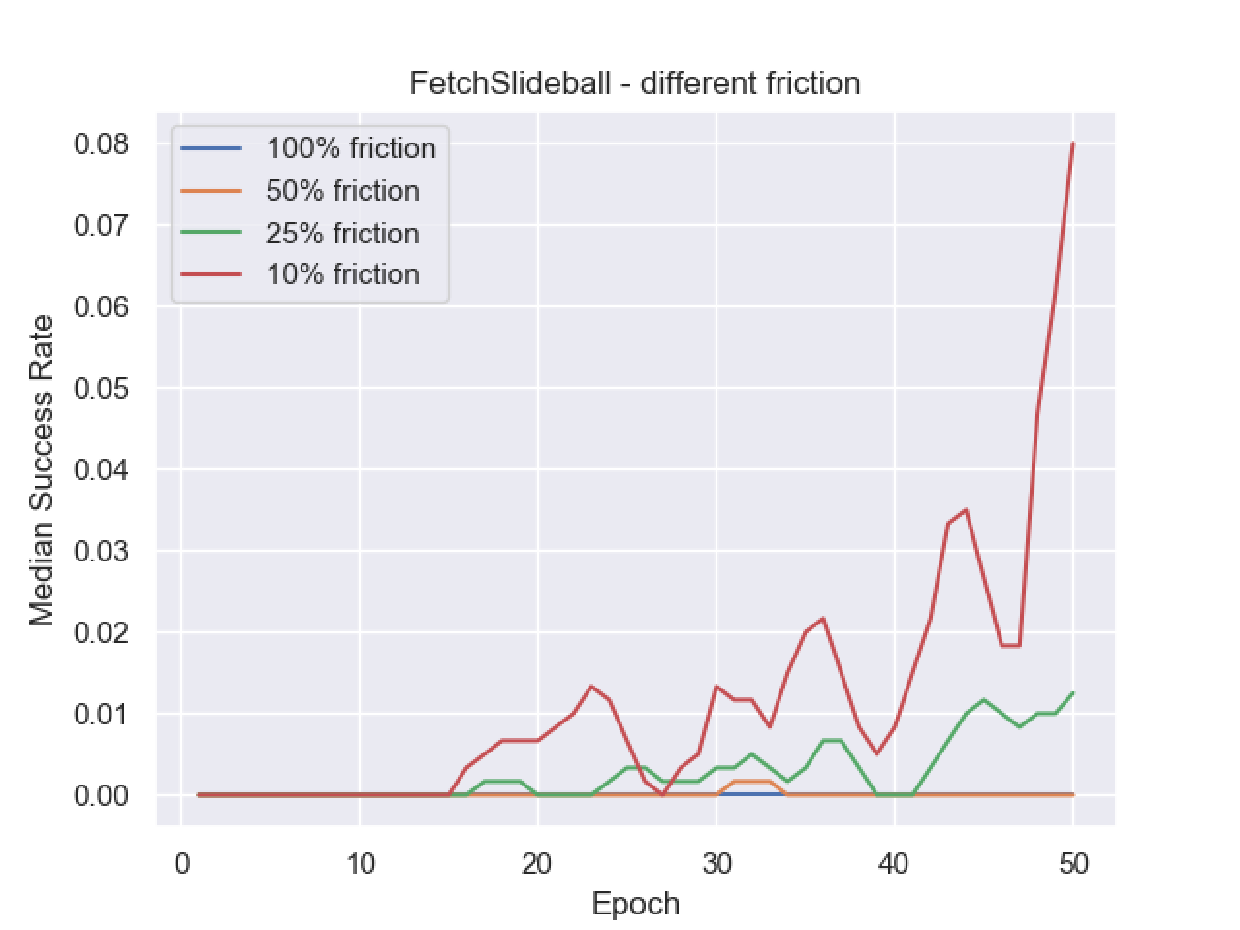
\includegraphics[width=0.5\paperwidth]{./Ressourcen/Figures/fig_FetchSlideball_friction.pdf}
	\end{textblock*}
	
	
	
	
	
\end{frame}
\clearpage

%%%%%%%%%%%%%%%%%%%%%%%%%%%%%%%%%%%%%%%%%%%%%%%%%%%%%%%%%%%%%%%%%%%%%%%%%%%%%%%%



% Seite 12


%%%%%%%%%%%%%%%%%%%%%%%%%%%%%%%%%%%%%%%%%%%%%%%%%%%%%%%%%%%%%%%%%%%%%%%%%%%%%%%%


\begin{frame}
	\frametitle{FetchToss}	
	\vspace{1cm}
	
	FetchToss-v1
	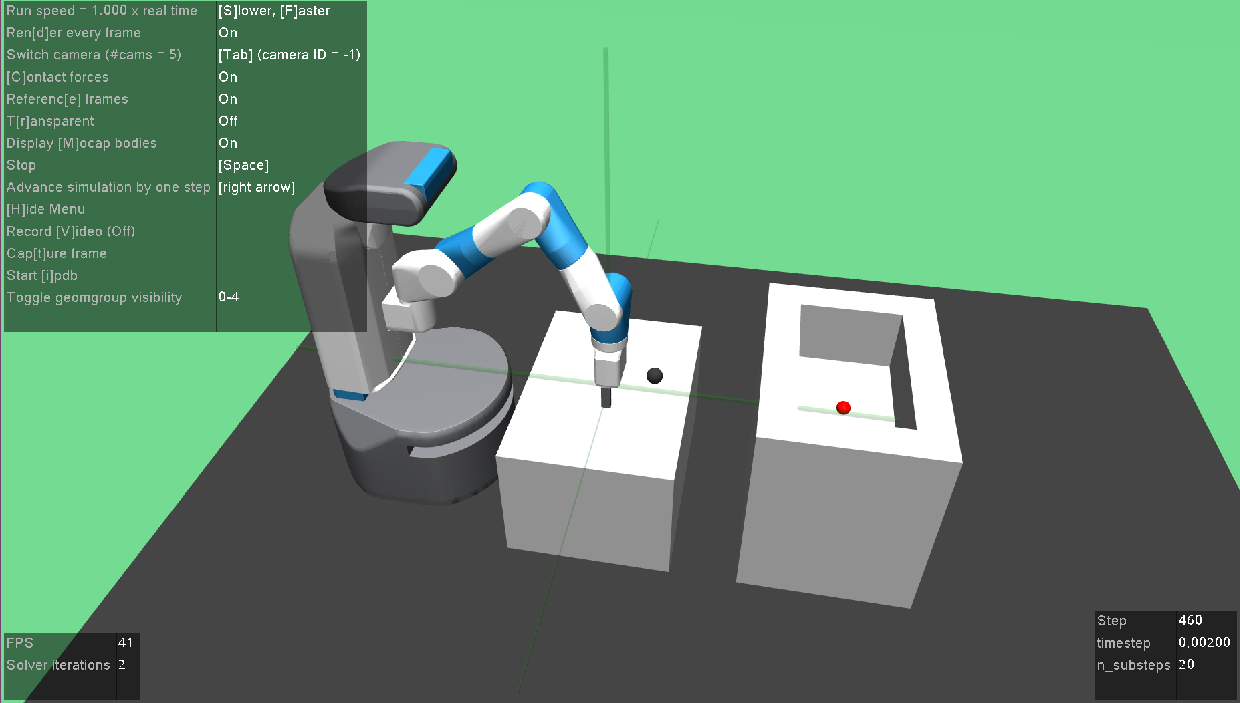
\includegraphics[width=\textwidth, height=.55\textheight]{./Ressourcen/Figures/FetchToss-v1.pdf}
	
\end{frame}
\clearpage




%%%%%%%%%%%%%%%%%%%%%%%%%%%%%%%%%%%%%%%%%%%%%%%%%%%%%%%%%%%%%%%%%%%%%%%%%%%%%%%%


% Seite 12.5

%%%%%%%%%%%%%%%%%%%%%%%%%%%%%%%%%%%%%%%%%%%%%%%%%%%%%%%%%%%%%%%%%%%%%%%%%%%%%%%%

\begin{frame}
	\frametitle{FetchPickAndPlaceball-v1}	
	\vspace{1cm}
	
	Same as FetchPickAndPlace-v1, but with a ball
	
	%Bild FetchSlide-v1
	
	\begin{textblock*}{0.5\paperwidth}[1,1](\textwidth + \PraesentationSeitenrand, 14cm - \PraesentationSeitenrand)%
		FetchPickAndPlaceball-v1 (ball)
		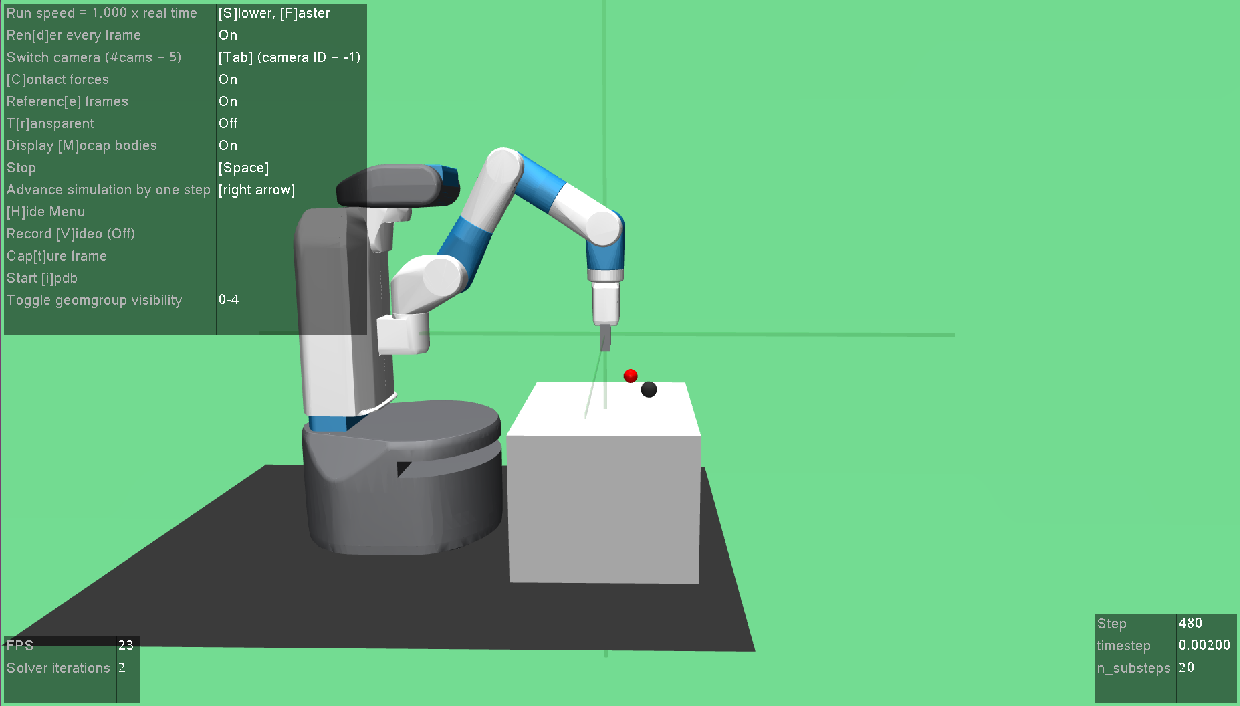
\includegraphics[width=0.4\paperwidth]{./Ressourcen/Figures/FetchPickAndPlaceball-v1.pdf}
	\end{textblock*}
	
	
	%Bild FetchSlideball-v1
	
	\begin{textblock*}{0.4\paperwidth}[0,1](0cm, 14cm - \PraesentationSeitenrand)%
		FetchPickAndPlace-v1 (cube)
		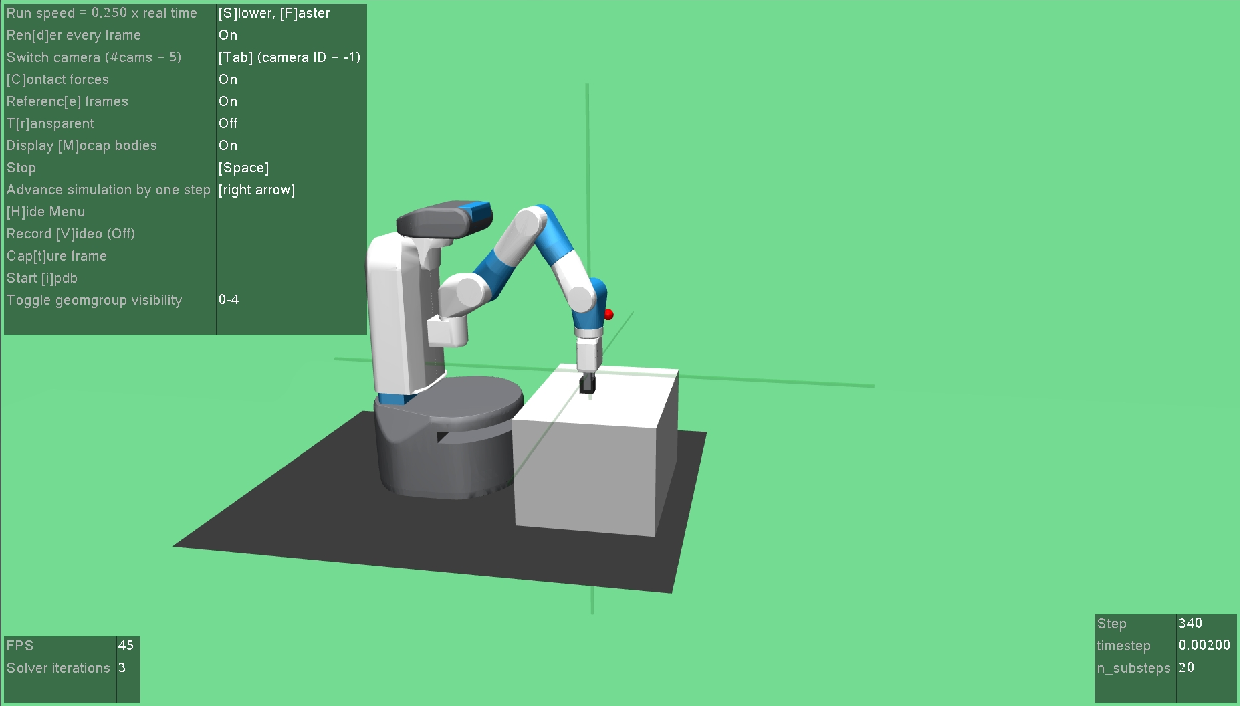
\includegraphics[width=0.4\paperwidth]{./Ressourcen/Figures/FetchPickAndPlace-v1.pdf}
	\end{textblock*}
	
	
	
	
\end{frame}
\clearpage

%%%%%%%%%%%%%%%%%%%%%%%%%%%%%%%%%%%%%%%%%%%%%%%%%%%%%%%%%%%%%%%%%%%%%%%%%%%%%%%%


% Seite 13


%%%%%%%%%%%%%%%%%%%%%%%%%%%%%%%%%%%%%%%%%%%%%%%%%%%%%%%%%%%%%%%%%%%%%%%%%%%%%%%%

\begin{frame}
	\frametitle{FetchPickAndPlaceball-v1}	
	\vspace{1cm}
	
	%Bild env
	\begin{textblock*}{0.4\paperwidth}[0,1](0cm, 13cm - \PraesentationSeitenrand)%
		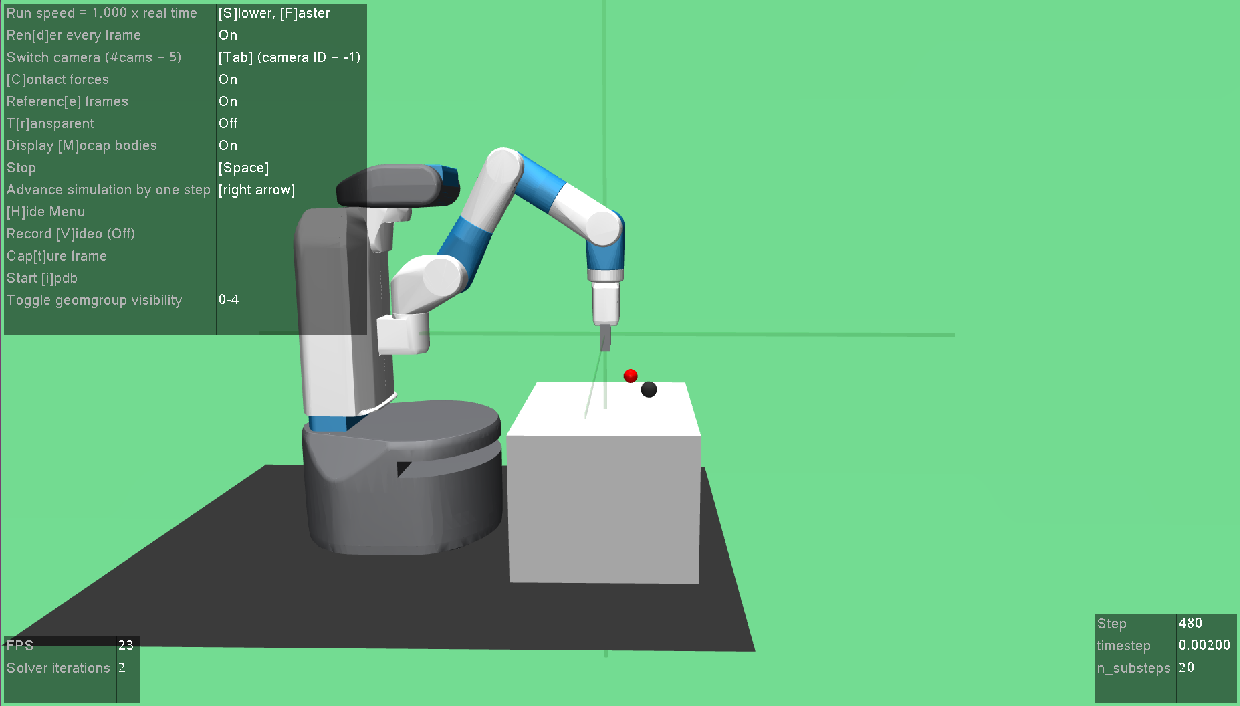
\includegraphics[width=0.4\paperwidth]{./Ressourcen/Figures/FetchPickAndPlaceball-v1.pdf}
	\end{textblock*}
	
	%Bild FetchPickAndPlace-v1 vs FetchPickAndPlaceball-v1
	\begin{textblock*}{0.5\paperwidth}[1,1](\textwidth + \PraesentationSeitenrand, 15cm - \PraesentationSeitenrand)%
		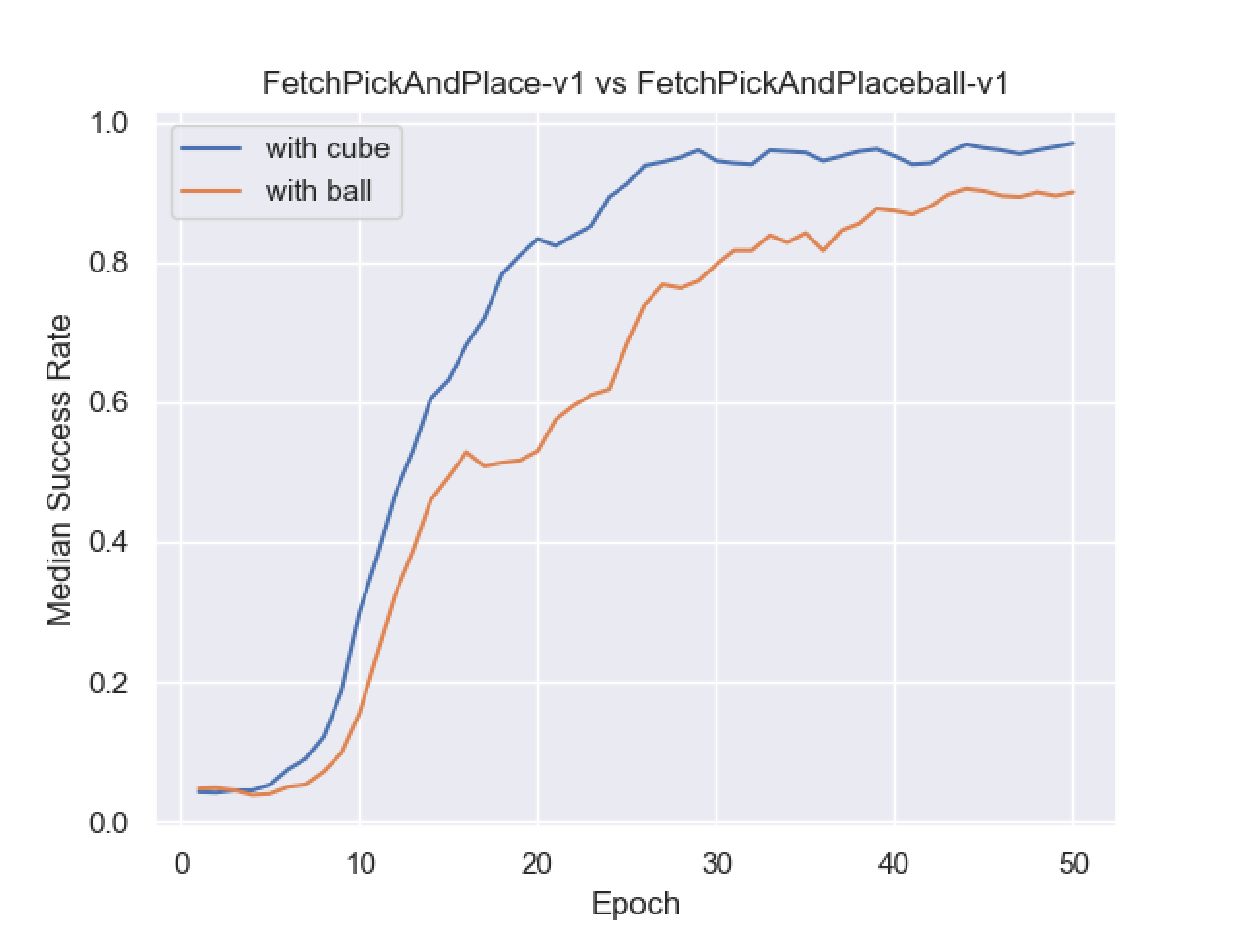
\includegraphics[width=0.5\paperwidth]{./Ressourcen/Figures/fig_FetchPickAndPlace-v1_vs_FetchPickAndPlaceball-v1.pdf}
	\end{textblock*}
	
	
\end{frame}
\clearpage

%%%%%%%%%%%%%%%%%%%%%%%%%%%%%%%%%%%%%%%%%%%%%%%%%%%%%%%%%%%%%%%%%%%%%%%%%%%%%%%%



% Seite 14


%%%%%%%%%%%%%%%%%%%%%%%%%%%%%%%%%%%%%%%%%%%%%%%%%%%%%%%%%%%%%%%%%%%%%%%%%%%%%%%%

\begin{frame}
	\frametitle{FetchToss Version 1-4}	
	\vspace{1cm}
	
	
	%Bild env
	\begin{textblock*}{0.4\paperwidth}[0,1](0cm, 16cm - \PraesentationSeitenrand)%
		
		Goal is only in the box \\
		Changes from v1 to v4: Better box, friction added, double steps/episode, 1\% weight
		
		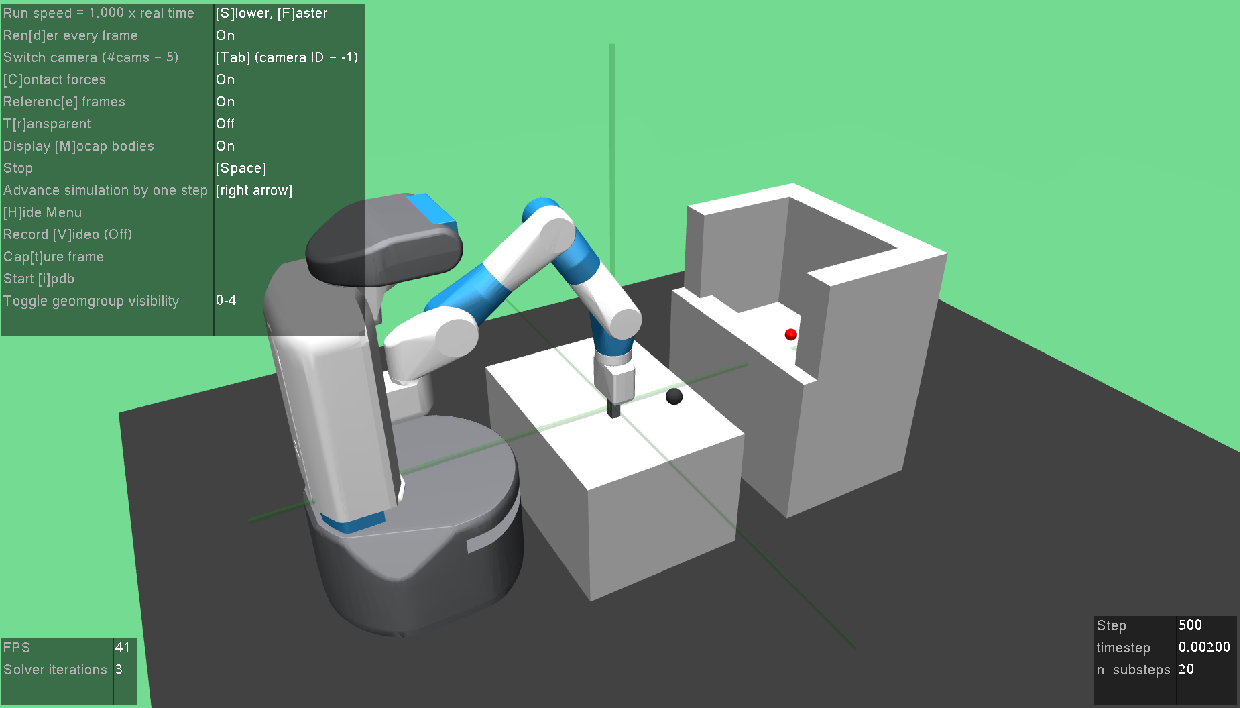
\includegraphics[width=0.4\paperwidth]{./Ressourcen/Figures/FetchToss-v3.pdf}
		
		
		
		-> Fail: because the goal is \textbf{only} in the box
		
	\end{textblock*}
	
	%Bild Success Rate
	\begin{textblock*}{0.5\paperwidth}[1,1](\textwidth + \PraesentationSeitenrand, 15cm - \PraesentationSeitenrand)%
		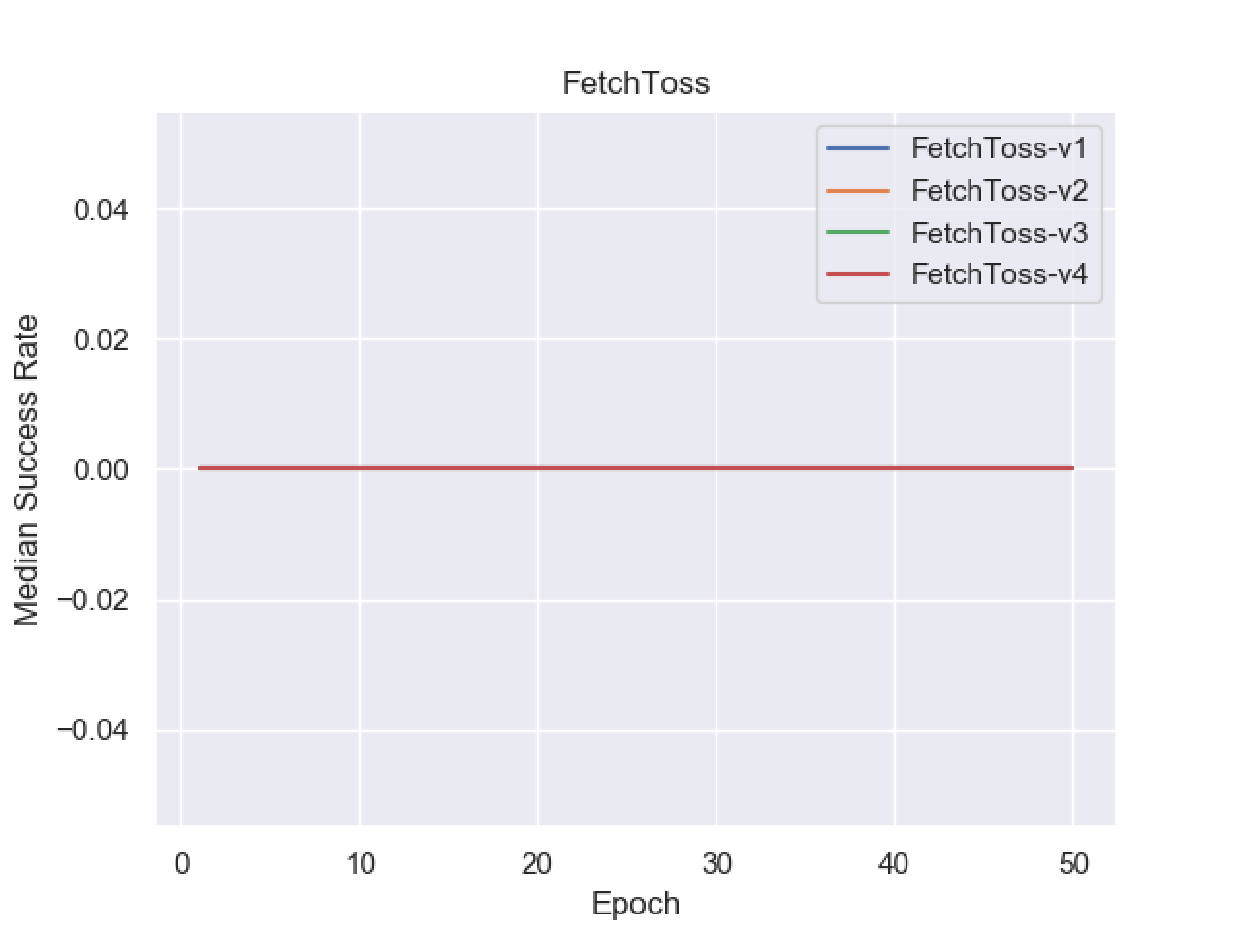
\includegraphics[width=0.5\paperwidth]{./Ressourcen/Figures/fig_FetchToss-v1-v4.pdf}
		

	\end{textblock*}
	
	

	
\end{frame}
\clearpage

%%%%%%%%%%%%%%%%%%%%%%%%%%%%%%%%%%%%%%%%%%%%%%%%%%%%%%%%%%%%%%%%%%%%%%%%%%%%%%%%





% Seite 15


%%%%%%%%%%%%%%%%%%%%%%%%%%%%%%%%%%%%%%%%%%%%%%%%%%%%%%%%%%%%%%%%%%%%%%%%%%%%%%%%

\begin{frame}
	\frametitle{FetchToss Version 5}	
	\vspace{1cm}
	
	%Bild env
	\begin{textblock*}{0.4\paperwidth}[0,1](0cm, 14cm - \PraesentationSeitenrand)%
		
		no friction, 1\% weight \\
		(25\% Toss, 75\% FetchPickAndPlace)
		
		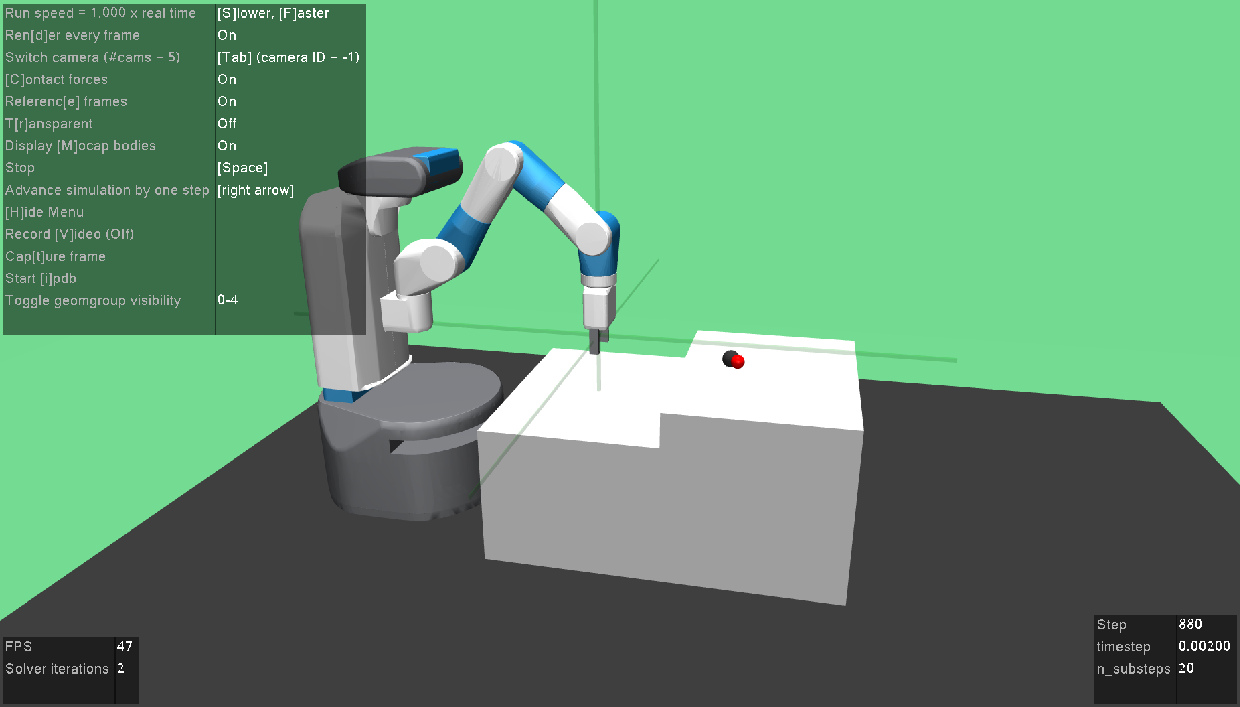
\includegraphics[width=0.4\paperwidth]{./Ressourcen/Figures/FetchToss-v5.pdf}
		
	\end{textblock*}
	
	%Bild Success Rate
	\begin{textblock*}{0.5\paperwidth}[1,1](\textwidth + \PraesentationSeitenrand, 15cm - \PraesentationSeitenrand)%
		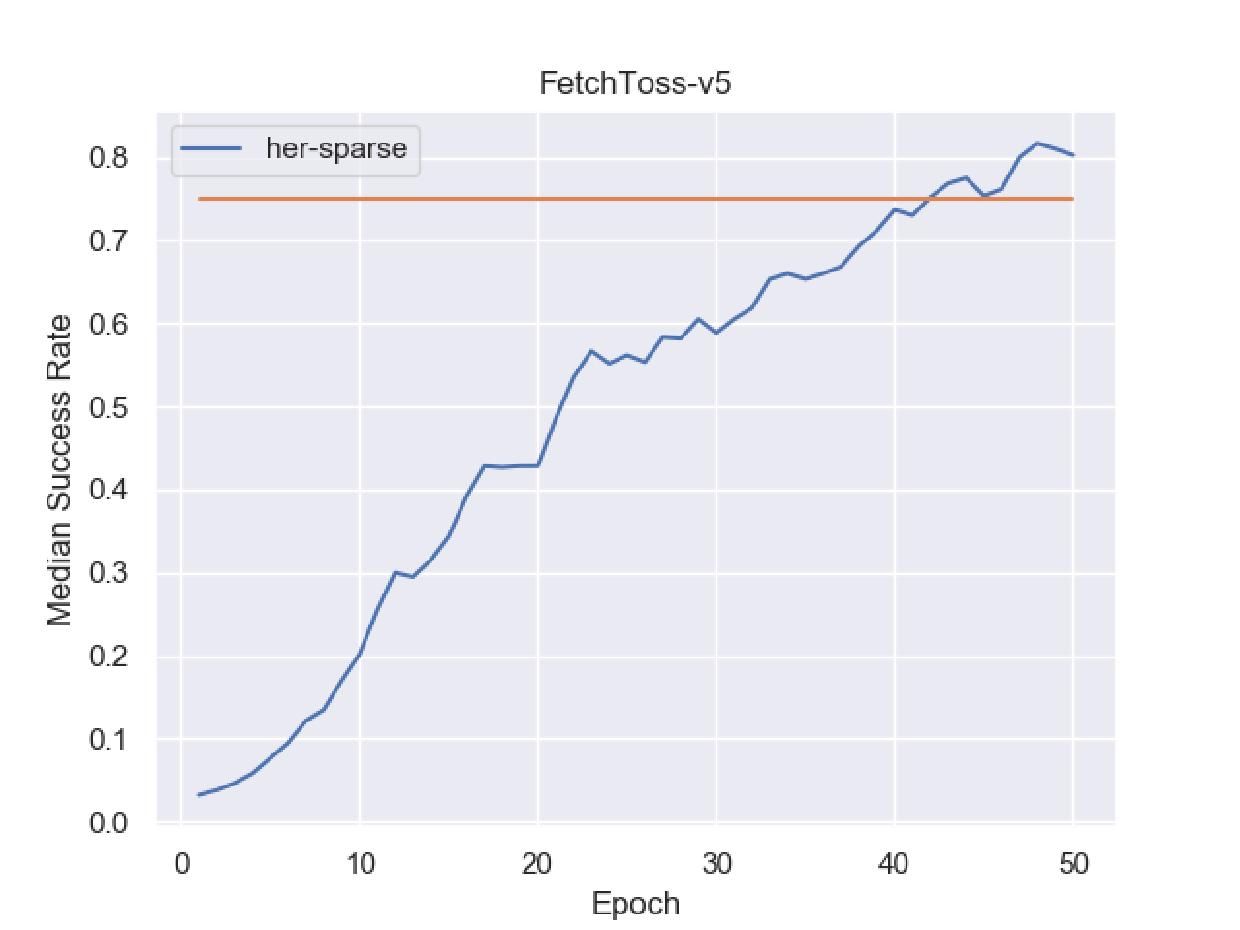
\includegraphics[width=0.5\paperwidth]{./Ressourcen/Figures/fig_FetchToss-v5.pdf}
		
		
	\end{textblock*}

	
\end{frame}
\clearpage

%%%%%%%%%%%%%%%%%%%%%%%%%%%%%%%%%%%%%%%%%%%%%%%%%%%%%%%%%%%%%%%%%%%%%%%%%%%%%%%%




% Seite 16


%%%%%%%%%%%%%%%%%%%%%%%%%%%%%%%%%%%%%%%%%%%%%%%%%%%%%%%%%%%%%%%%%%%%%%%%%%%%%%%%

\begin{frame}
	\frametitle{FetchToss with different height}	
	\vspace{1cm}
		
		
	%Bild env
	\begin{textblock*}{0.4\paperwidth}[0,1](0cm, 14cm - \PraesentationSeitenrand)%
		FetchToss-v13 (height: 0.7)
		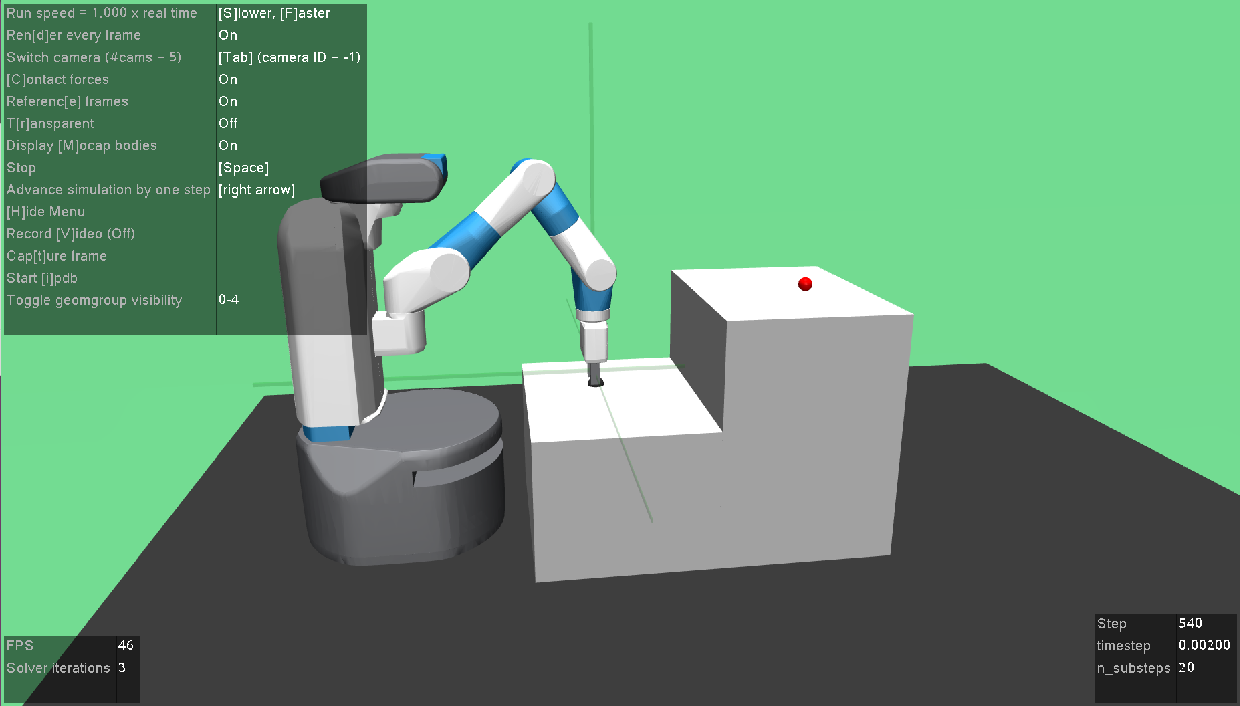
\includegraphics[width=0.4\paperwidth]{./Ressourcen/Figures/FetchToss-v13.pdf}
		
	\end{textblock*}
	
	%Bild Success Rate
	\begin{textblock*}{0.5\paperwidth}[1,1](\textwidth + \PraesentationSeitenrand, 15cm - \PraesentationSeitenrand)%
		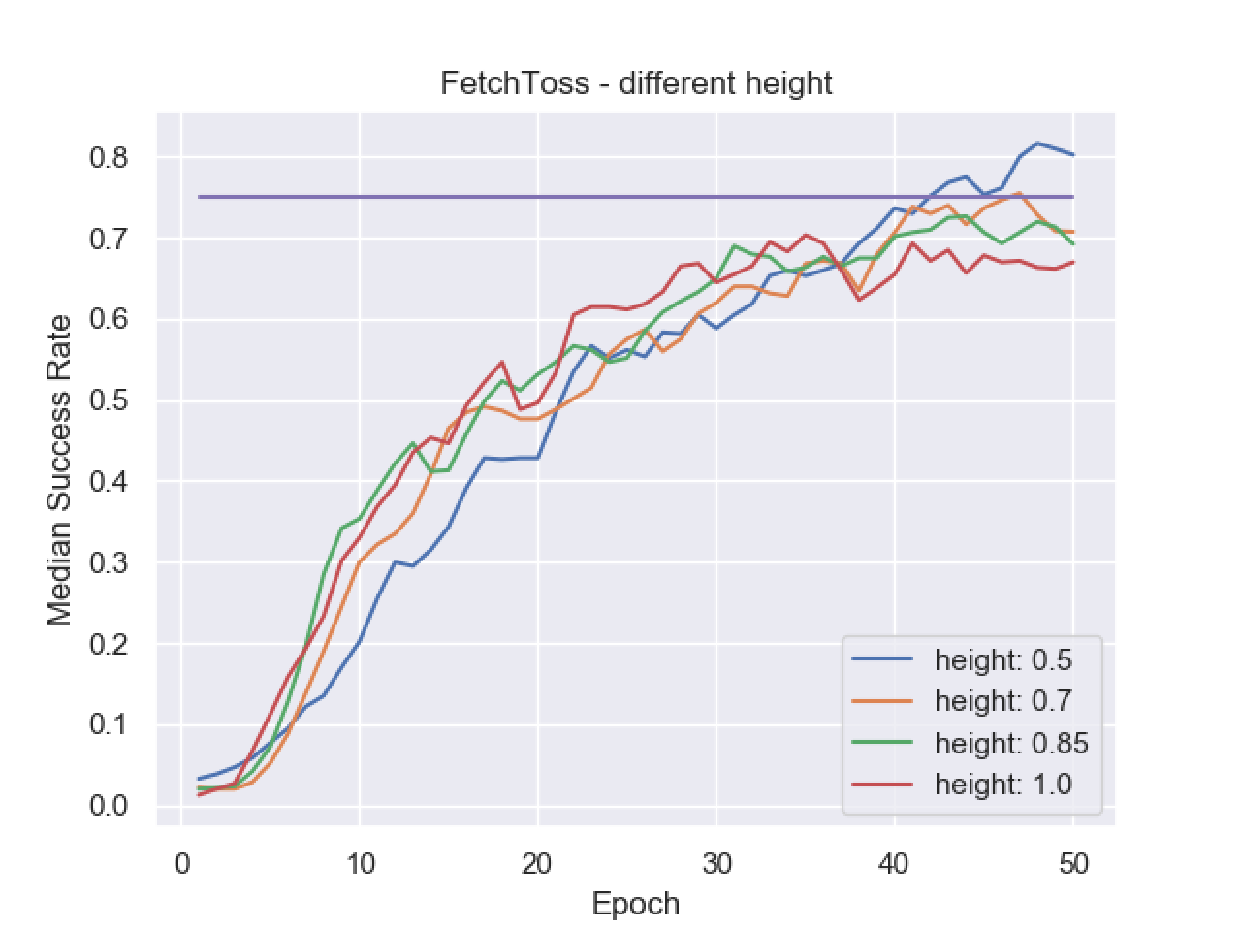
\includegraphics[width=0.5\paperwidth]{./Ressourcen/Figures/fig_FetchToss_height.pdf}
		
		
	\end{textblock*}
		
	%Bild env
	
\end{frame}
\clearpage

%%%%%%%%%%%%%%%%%%%%%%%%%%%%%%%%%%%%%%%%%%%%%%%%%%%%%%%%%%%%%%%%%%%%%%%%%%%%%%%%


% Seite 17


%%%%%%%%%%%%%%%%%%%%%%%%%%%%%%%%%%%%%%%%%%%%%%%%%%%%%%%%%%%%%%%%%%%%%%%%%%%%%%%%

\begin{frame}
	\frametitle{FetchToss with different weight}	
	\vspace{1cm}
	
	goal distance is longer
	
	%Bild env
	\begin{textblock*}{0.4\paperwidth}[0,1](0cm, 14cm - \PraesentationSeitenrand)%
		FetchToss-v10 (weight: 1\%)
		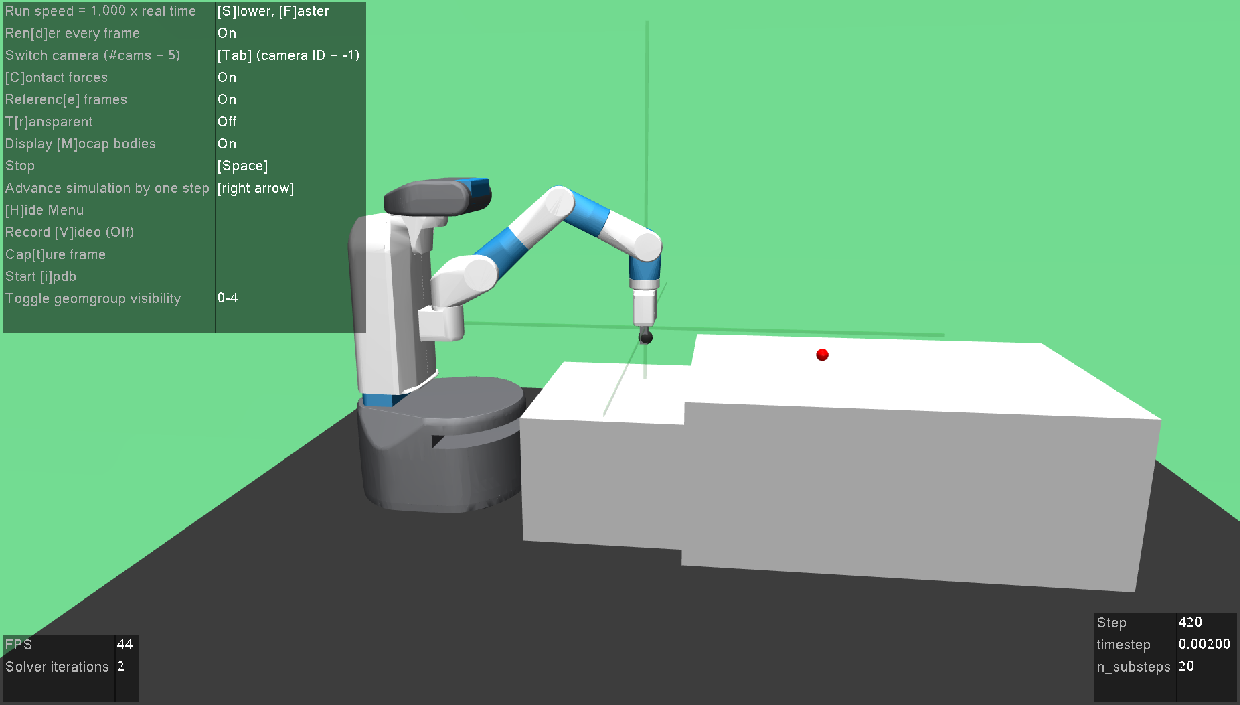
\includegraphics[width=0.4\paperwidth]{./Ressourcen/Figures/FetchToss-v10.pdf}
		
	\end{textblock*}
	
	
	%Bild Success Rate
	\begin{textblock*}{0.5\paperwidth}[1,1](\textwidth + \PraesentationSeitenrand, 15cm - \PraesentationSeitenrand)%
		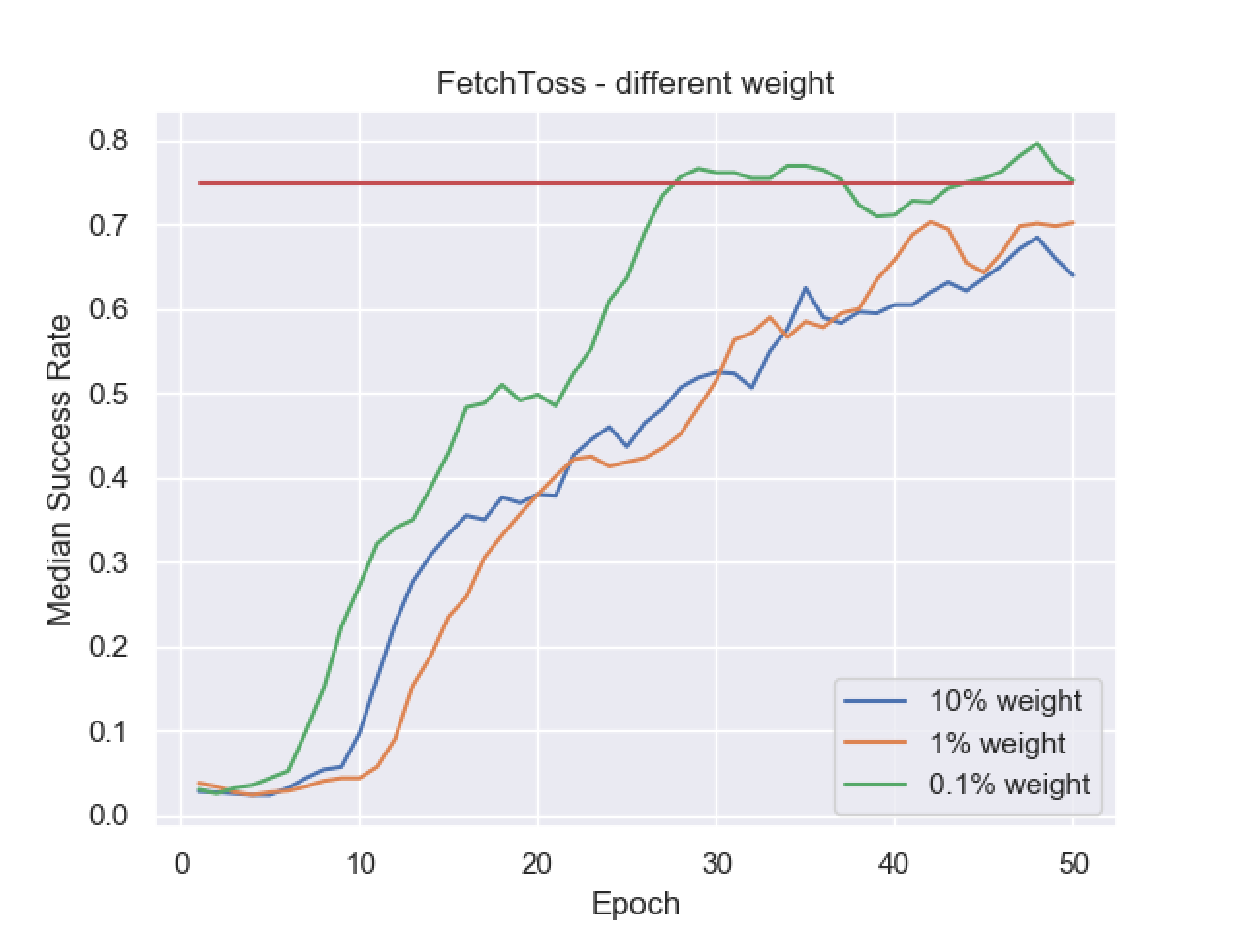
\includegraphics[width=0.5\paperwidth]{./Ressourcen/Figures/fig_FetchToss_weight.pdf}
	\end{textblock*}	
	
	
\end{frame}
\clearpage

%%%%%%%%%%%%%%%%%%%%%%%%%%%%%%%%%%%%%%%%%%%%%%%%%%%%%%%%%%%%%%%%%%%%%%%%%%%%%%%%

 
% Seite 18


%%%%%%%%%%%%%%%%%%%%%%%%%%%%%%%%%%%%%%%%%%%%%%%%%%%%%%%%%%%%%%%%%%%%%%%%%%%%%%%%

\begin{frame}
	\frametitle{Conclusion and Future Work}	
	\vspace{1cm}
	
    \begin{PraesentationAufzaehlung}
    	\item Tossing in general works
    	\item Struggle to toss up and long distances \\
        \vspace{\baselineskip}
    	\underline{Ideas for Future Works:}
    	\item Try different parameters
    	\item Different gripper (more human-like hand)
    	\item Obstacles between robotic arm and goal
    	\item Different Objects (paper plane)


    	
    \end{PraesentationAufzaehlung}
    
	
\end{frame}
\clearpage

%%%%%%%%%%%%%%%%%%%%%%%%%%%%%%%%%%%%%%%%%%%%%%%%%%%%%%%%%%%%%%%%%%%%%%%%%%%%%%%%










%%%%%%%%%%%%%%%%%%%%%%%%%%%%%%%%%%%%%%%%%%%%%%%%%%%%%%%%%%%%%%%%%%%%%%%%%%%%%%%%


\begin{frame}
	\frametitle{Presentation Sources}	
	\vspace{1cm}
	
	https://blog.goodaudience.com/what-is-inverse-reinforcement-learning-e333228af146
	
	https://pixabay.com/de/photos/basketball-net-ergebnis-felge-2099656/
	
	https://pixabay.com/de/photos/golf-golfball-loch-golfplatz-pokal-1284012/
	
	https://en.wikipedia.org/wiki/Paper\_Toss/
	
	
\end{frame}
\clearpage


%%%%%%%%%%%%%%%%%%%%%%%%%%%%%%%%%%%%%%%%%%%%%%%%%%%%%%%%%%%%%%%%%%%%%%%%%%%%%%%%


\end{document} % !!! NICHT ENTFERNEN !!!
%%%%%%%%%%%%%%%%%%%%%%%%%%%%%%%%%%%%%%%%%%%%%%%%%%%%%%%%%%%%%%%%%%%%%%%%%%%%%%%%
